\documentclass[a4paper]{report}
\usepackage{amsmath}
\usepackage{amssymb}
% for pseudo code
\usepackage{algorithm,algpseudocode}
%
\usepackage{ulem}
\usepackage{ngerman}
\usepackage{graphicx}
\usepackage{subfig}
\usepackage[svgnames]{xcolor} % Required for colour specification
\newcommand*{\plogo}{\fbox{$\mathcal{PL}$}} % Generic dummy publisher logo
\renewcommand{\baselinestretch}{1.25}
\usepackage[T1]{fontenc} % Output font encoding for international characters
\usepackage[utf8]{inputenc} % Required for inputting international characters
\usepackage{tgadventor} % Use the Paratype Serif font
\renewcommand{\familydefault}{\sfdefault}
\usepackage{float}
\usepackage{tcolorbox}
\usepackage[hidelinks]{hyperref}
\usepackage{refstyle}
\usepackage{caption}
\usepackage{pdfpages}%
\usepackage{geometry}
 \geometry{
 left=30mm,
 top=30mm,
 bottom=20mm,
 }

\usepackage{fancyhdr}
\pagestyle{fancy}
\fancyhf{}
\rhead{MBE}
%\lhead{\LaTeX{} tutorials}
\lhead{\nouppercase{\rightmark} (\nouppercase{\leftmark})}
\rfoot{Page \thepage}
\renewcommand{\headrulewidth}{2pt}


\usepackage{listings}

	%------------------------------------------------
	%	Start der Beschreibung
	%------------------------------------------------
\begin{document}


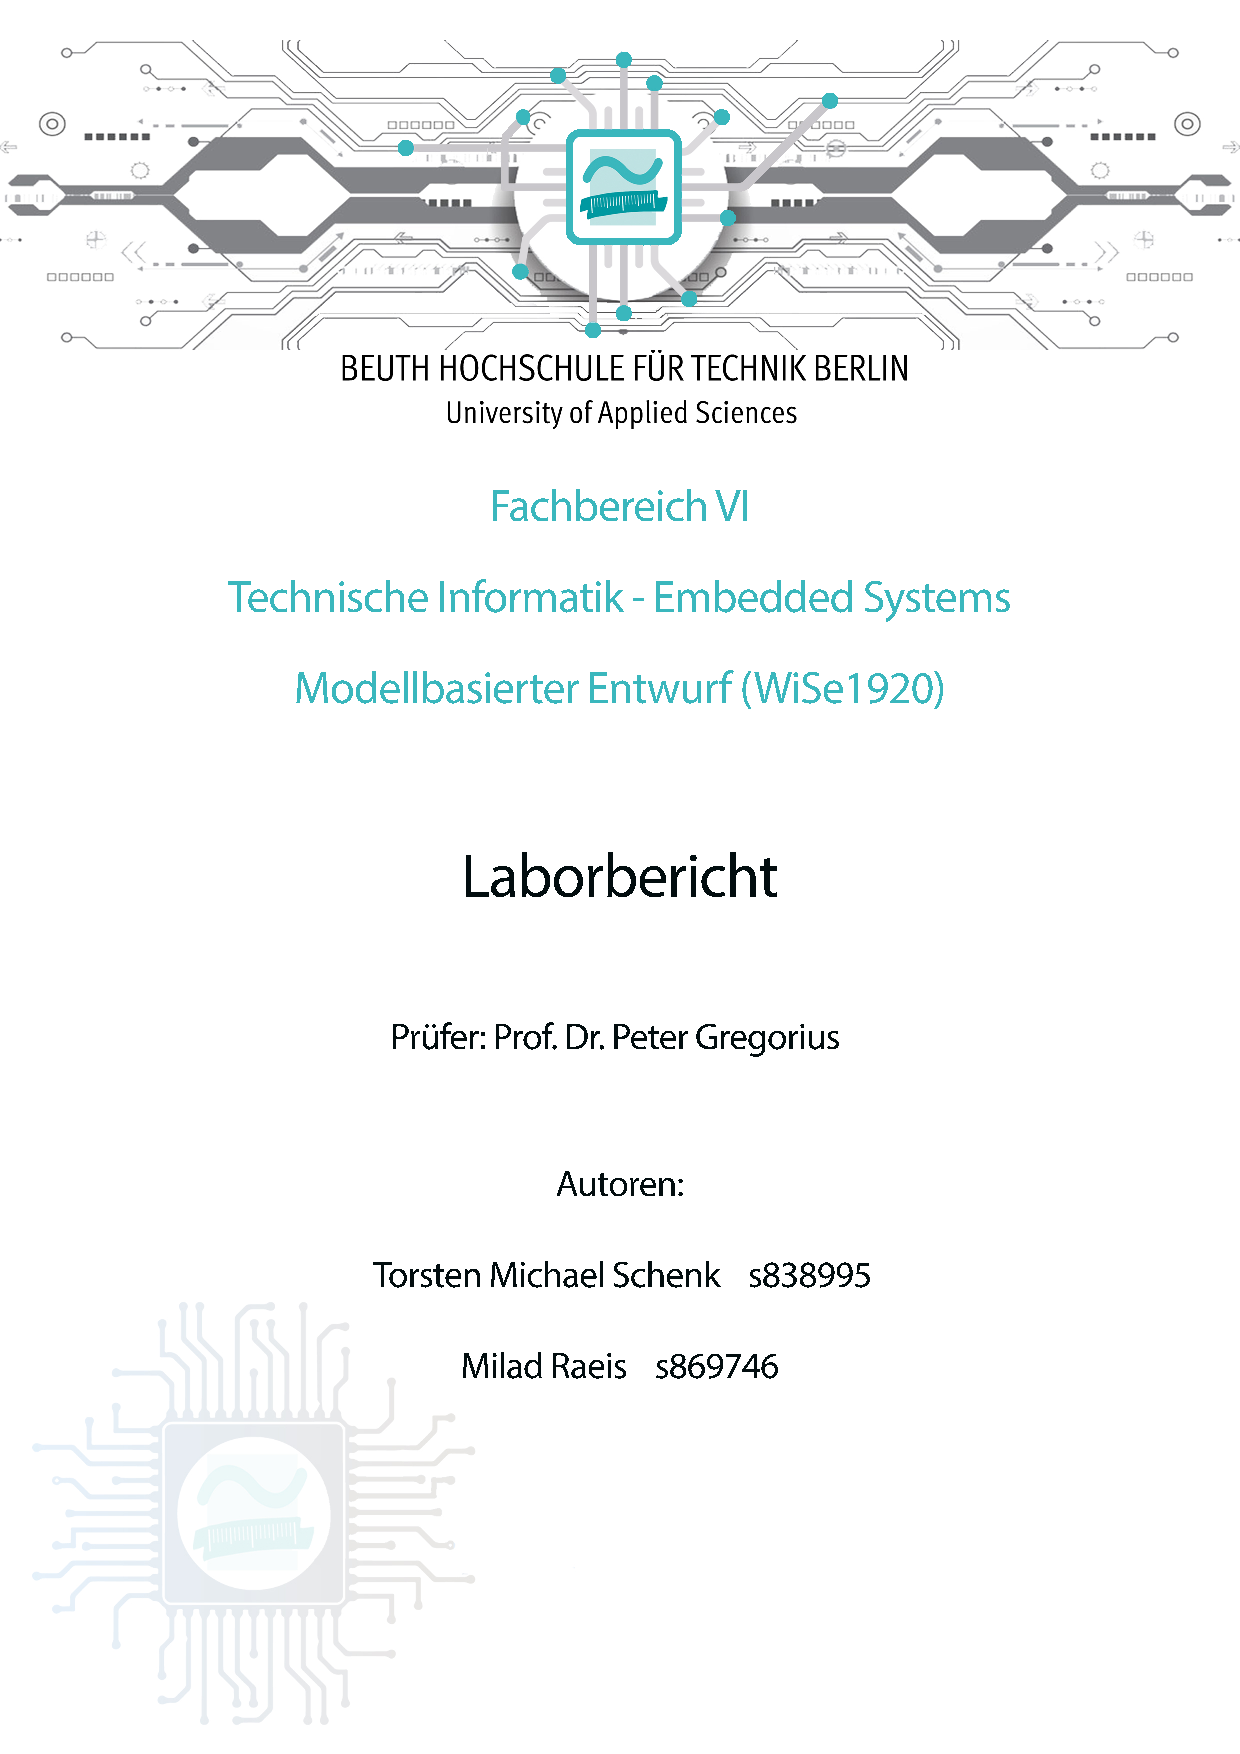
\includepdf{Coverpage.pdf}
\tableofcontents
\listoffigures




\section{Vorwort}
Bei der Recherche zur Bearbeitung der Übungen wurden viele englischsprachige Webseiten zu rate gezogen. Generell kann man sagen, dass englische Fachbegriffe sich im Bereich FPGA und embedded Design etabliert haben, so dass eine Übersetzung eher verwirren als helfen würde. Daher haben wir uns entschieden, die \textbf{englischen} Bezeichner und Beschreibungen beizubehalten.\\
Um Codeabschnitte besser von Beschreibungen besser unterscheiden zu können, wurde eine eigene Schriftart verwendet:
\begin{verbatim}
  Kommandozeilen Eingaben und Codesnippets werden wie HIER dargestellt.
\end{verbatim}

\chapter{Projektbeschreibung}
\label{Projektbeschreibung}
In diesem Projekt sollen die Momente von Regionen (Blobs) berechnet werden. Momente sind im englischen Sprachgebrauch etabliert und werden im Deutschen als Massenträgheitsmomente oder einfach Trägheitsmomente bezeichnet. Sie kommen zum Einsatz wo statische Kennwerte die Konturabhängig sind benötigt werden. Eine wichtige Fragestellung ist z.B. in welcher Richtung sich ein L-Profil biegen wird. Die kontinuierliche Darstellung von Momenten als Integral in dem I(x,y) die gesamte Fläche eines Querschnittes darstellt: $$M = \int \int I(i,j) dxdy$$

Diskret (Bildpixel) können durch Iteration über alle Pixel einer Region die Momente berechnet werden. Die allgemeine Formel kann für alle Kombinationen verwendet werden, z.B. $M_{00}$, $M_{01}$, $M_{20}$. Die Zahlen dienen hierbei gleichzeitig als Exponent p oder q.: $$M_{p,q} = \sum \sum i^p jp^q I(i,j)$$

	\begin{figure}[H]
	\centering
	\subfloat{
\includegraphics[width=9cm,height=6cm]{PIC/cbwimg}}
	\caption{Beispiel: binarisiertes Bild}
	\label{Entwurf des Projects}
	\end{figure}

Im Projekt soll auf Bildern jeweils mindestens eine Region selektiert werden. In diese soll zur Anzeige des Ergebnisses der Schwerpunkt und die Orientierung in Richtung der Achse mit höherem Biegemoment. In der folgenden Abbildung sind die Schwerpunkte lila und die Orientierung grün eingezeichnet.
	
	\begin{figure}[H]
	\centering
	\subfloat{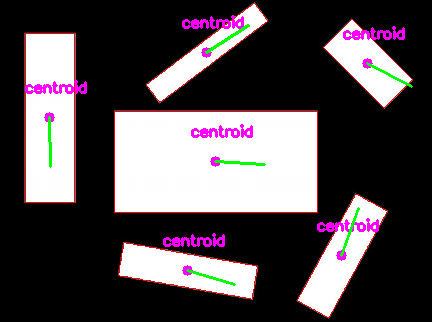
\includegraphics[width=9cm,height=6cm]{PIC/colorres}}
	\caption{Beispiel: Blobs mit Schwerpunkt und Richtung}
	\label{Entwurf des Projects}
	\end{figure}
	
Nach der binarisierung der Region können die Pixel jeder Region gezählt werden und sind in x und y Koordinaten im Bild bekannt. Zuerst werden die Schwerpunkte $\overline{x}$ und $\overline{y}$ berechnet. Danach erfolgt die Berechnung der Orientierung aus den Flächenmomenten mittels der Kovarianzen und der Kovarianzmatrix. \\

Schwerpunkt x: $$\overline{x} = \frac{M_{10}}{M_{00}}$$

Schwerpunkt y: $$\overline{y} = \frac{M_{01}}{M_{00}}$$

Kovarianzen: $$\mu_{11} = \frac{M_{11}}{M_{00}} - \overline{x}\overline{y} $$
			 $$\mu_{02} = \frac{M_{02}}{M_{00}} - \overline{y}^2 $$
			 $$\mu_{20} = \frac{M_{20}}{M_{00}} - \overline{x}^2 $$

     		$$cov(Obj) =\begin{bmatrix}
			 			\mu_{20} & \mu_{11}\\ 
				 		\mu_{11}& \mu_{02}
					 	\end{bmatrix}$$
			
			 
Orientierung einer Region im Wertebereich (+$\pi$, -$\pi$): $$ \theta = \frac{1}{2} atan2(2\mu_{11}, (\mu_{20}-\mu_{02}))    $$

Bei der Hardware Realisierung sind mehrere Optionen denkbar. Es werden FPGA Implementation für Kamera via PMOD und VGA über SHIELD PINs angestrebt. Sollte sich der mathematische Teil als \textbf{semesterfüllend} herausstellen, kann auf USB Kamera und HDMI Display (Anbindung über Pynq-Linux) ausgewichen werden. Im Worse-Case wäre noch das Laden und Speichern von Bildern aus einem Bildordner als Möglichkeit offen. \textbf{Im Vordergrund steht die Implementation der mathematischen Funktionen deren Verarbeitung im FPGA erfolgt.}

	%------------------------------------------------
	%	1. Chapter
	%------------------------------------------------

\chapter{Hardware}

In diesem Kapitel wird die für das Projekt erforderliche Hardware dargestellt und erläutert. Optional kann im Projekt die Kamera auf zwei verschiedene Arten angeschlossen werden. Die erste Möglichkeit ist über Verwendung des HDMI-Ports einen Bilschirm anzuschließen:
	\begin{figure}[H]
	\centering
	\subfloat{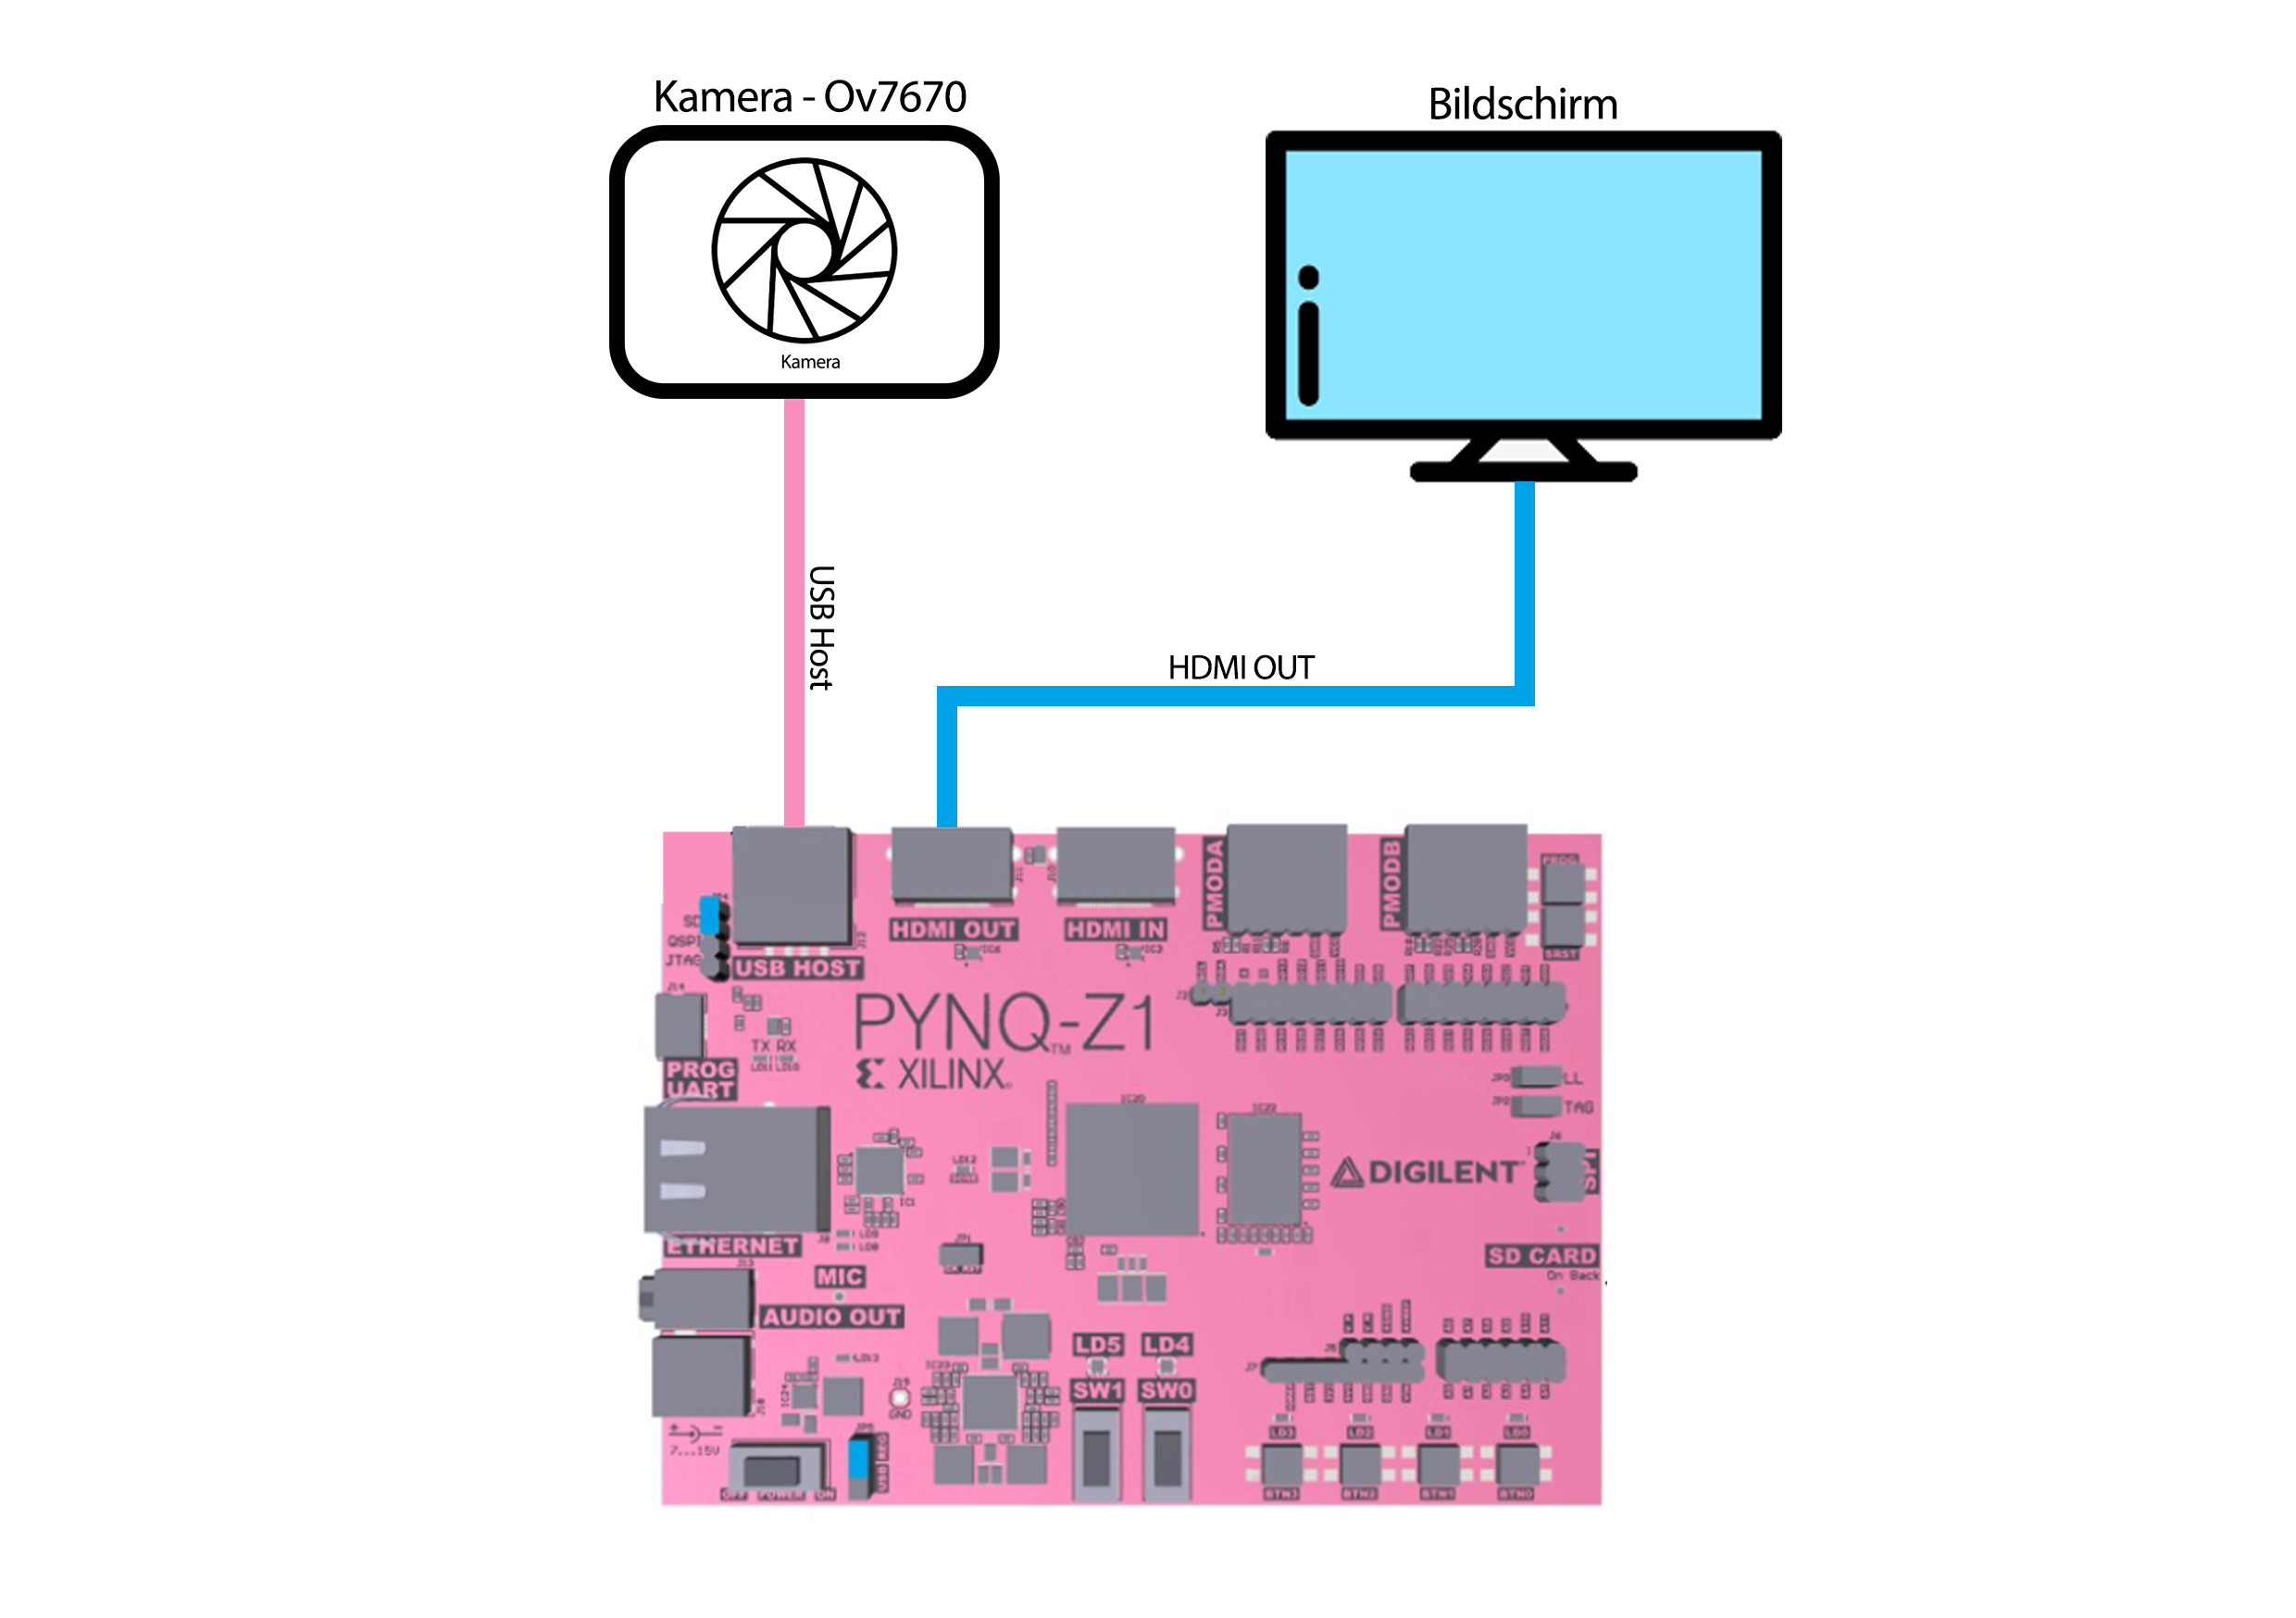
\includegraphics[width=15cm,height=9cm]{PIC/schematikcameraUsb}}
	\caption{Entwurf des Projects durch USB Host und HDMI OUT}
	\label{Entwurf des Projects durch_USB_Host_und_HDMI_OUT}
	\end{figure}

Die zweite Möglichkeit, wie unten im Entwurf gezeigt, wir über die FPGA Pins mit VGA Adapter ein Bildschirm angeschlossen.
	\begin{figure}[H]
	\centering
	\subfloat{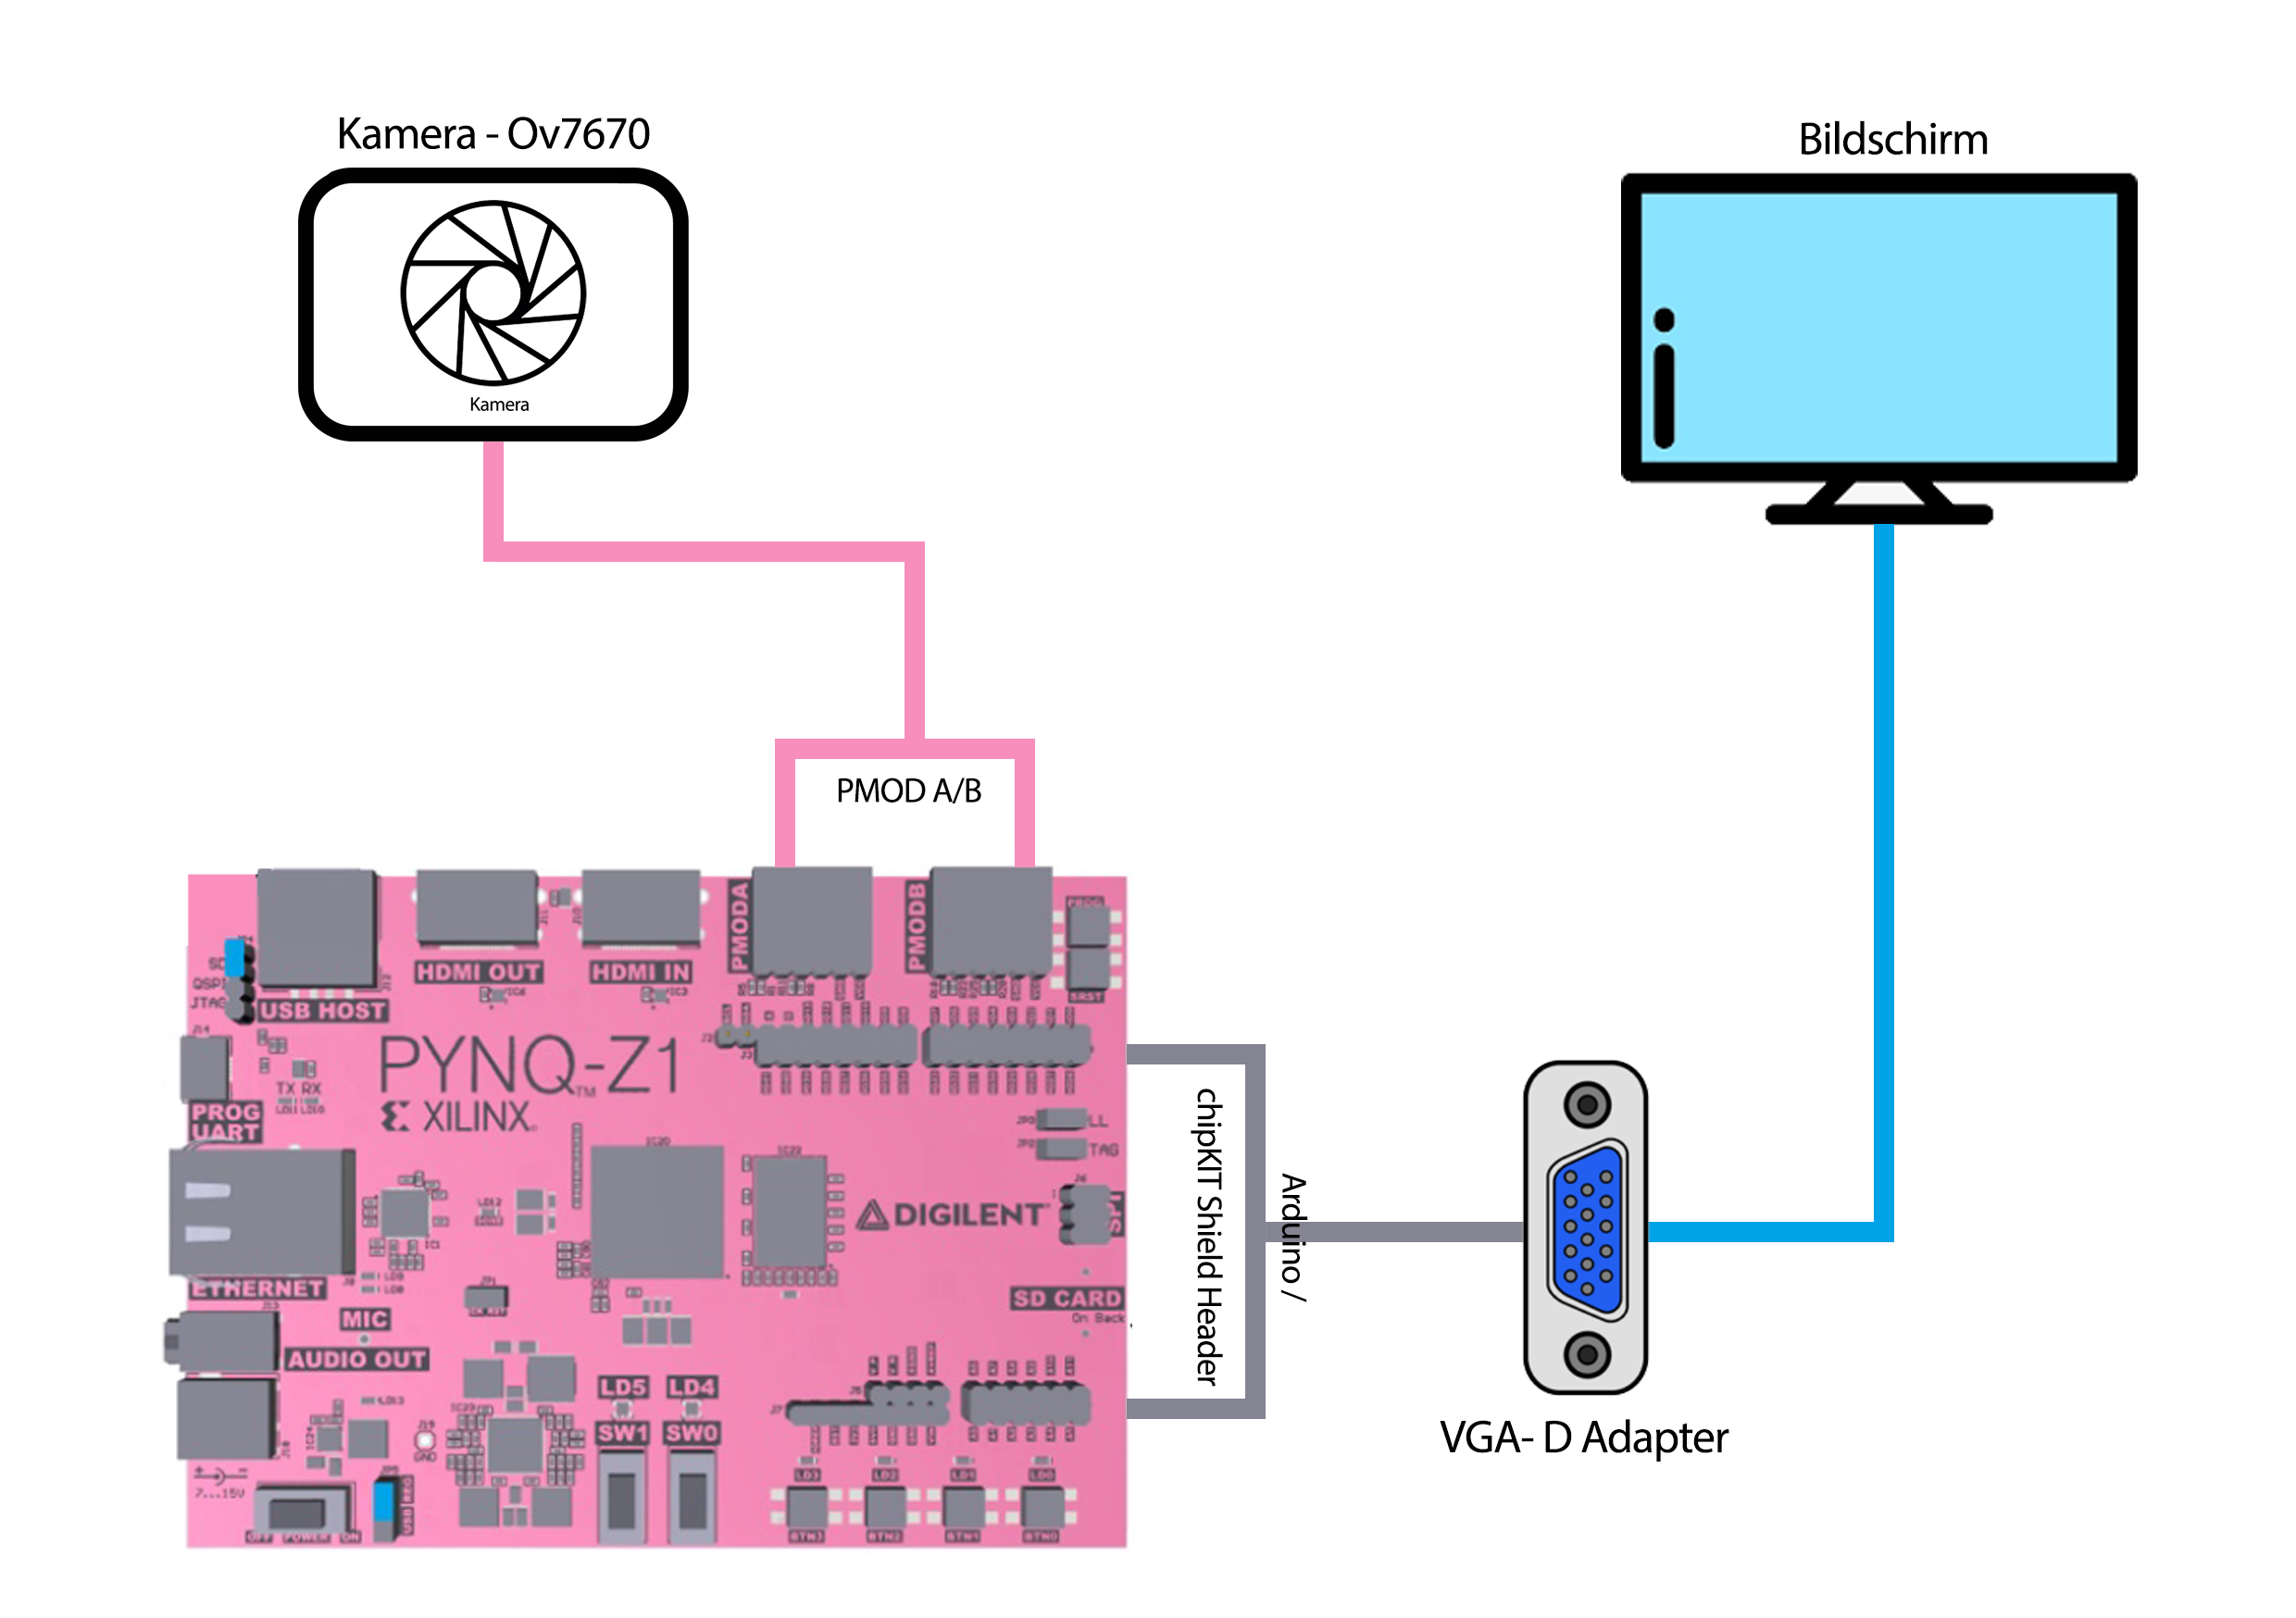
\includegraphics[width=13cm,height=8cm]{PIC/schematik}}
	\caption{Entwurf des Projects durch VGA Adapter}
	\label{Entwurf des Projects durch_VGA_Adapter}
	\end{figure}
	
Die Kamera kann ebenfalls entweder an USB oder PMOD...


\section{Xilinx Pynq-Z1 board}
Das PYNQ-Z1 Board wurde für die Verwendung mit PYNQ entwickelt, einem neuen Open-Source-Framework, das es Embedded-Programmierern ermöglicht, die Fähigkeiten von Xilinx Zynq All Programmable SoCs\footnote{System On Chip} (APSoCs) zu nutzen, ohne programmierbare Logikschaltungen entwickeln zu müssen. Die programmierbaren Logikschaltungen werden als Hardwarebibliotheken importiert und  ihre APIs\footnote{Application Programming Interface} sind im Wesentlichen so programmiert, dass sie wie die Softwarebibliotheken importiert und programmiert werden. Für Designer, die das Basissystem mit neuen Hardware-Bibliotheken erweitern wollen, stehen die Xilinx Vivado WebPACK-Tools kostenlos zur Verfügung.

Das PYNQ-Z1 unterstützt Multimedia-Anwendungen mit integrierten Audio- und Videoschnittstellen und ist so konzipiert, dass es unkompliziert mit Pmod-, Arduino- und Grove-Peripheriegeräten sowie universellen IO-Pins erweiterbar ist.
Ebenso kann das PYNQ-Z1 Board auch mit USB-Peripheriegeräten wie WiFi, Bluetooth und Webcams erweitert werden und ist die Hardware-Plattform für das PYNQ Open-Source-Framework.

	\begin{figure}[H]
	\centering
	\subfloat{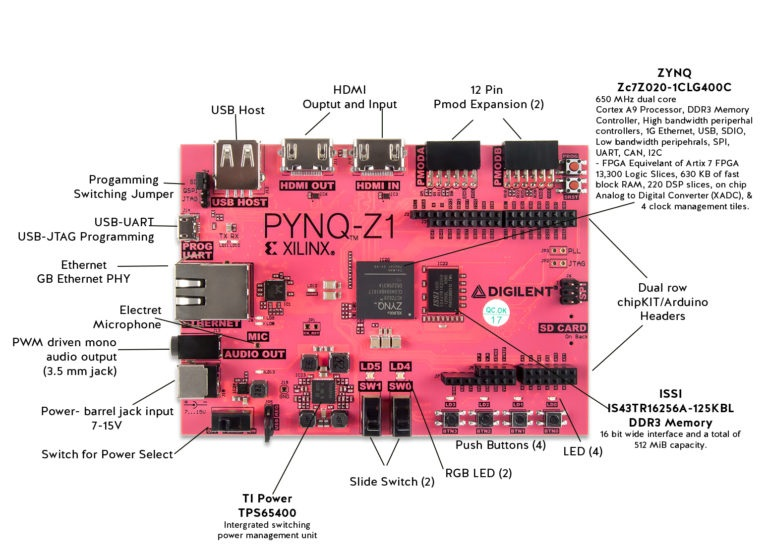
\includegraphics[width=15cm,height=9cm]{PIC/PYNQZ1}}
	\caption{Übersicht PYNQ-Z1}
	\label{Übersicht PYNQ-Z1}
	\end{figure}

Hardwarekomponenten auf dem Pynq-Z1 Board:

	\begin{enumerate} 
	\item 512 MB DDR3 mit 16-bit Bus bei 1050Mbps.
	\item 650 MHz Dual-Core Cortex-A9 Prozessor.
	\item 16 MB Quad-SPI\footnote{Serial Peripheral Interface} Flash, werkseitig programmiertem.
	\item Peripherie-Controller mit niedriger Bandbreite: SPI, UART, KANN, I2C.
	\item 630 KB fast block RAM.
	\item13,300 Logikscheiben mit je vier 6 Eingangs-LUT und 8 Flip-Flops.
	\item u.s.w\\
	\end{enumerate}

\subsection{PYNQ Z1 Core}
Das PYNQ-Z1 besteht aus einem Zynq-XC7Z020-1CLG400C (xc7z020dg400-1) SoC, der wiederum einen dual Core ARM Cortex-A9 und einen Artix-7 FPGA enthält:

	\begin{figure}[H]
	\centering
	\subfloat{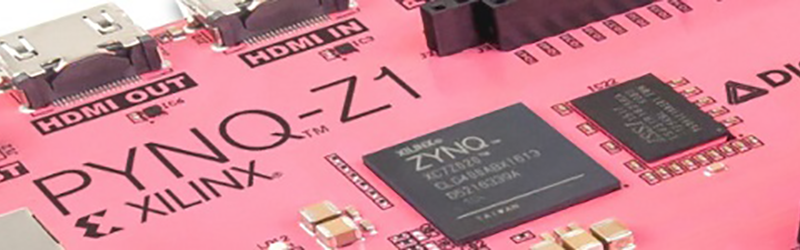
\includegraphics[width=8cm]{PIC/pynqcore}}
	\caption{PYNQ Z1 Core}
	\label{PYNQ Z1 Core}
	\end{figure}


\subsection{Power Jumper}

PYNQ Z1 hat 2 \textbf{''Modi''} Formen der Spannungsversorgung. Die Modi werden durch die Änderung des Power Jumpers JP5 gewählt.

\begin{enumerate} 
\item \textbf{USB} über Anschluss J14 (PROG oder UART)
\item  \textbf{REG} über Anschluss J18 (External Power)\\
\end{enumerate}

\textbf{Hinweis1 :} Die Ausgangsspannung \textbf{AC} muss zwischen 7VDC und 15VDC sein.
	
\textbf{Hinweis2 :} Wenn die Eingangsspannungen \textbf{>15VDC} sein, wird das Board beschädigt.



	\begin{figure}[H]
	\centering
	\subfloat{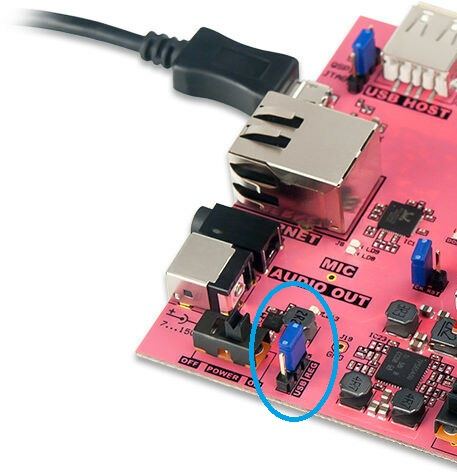
\includegraphics[width=5cm]{PIC/Jumper_Netzteil}}
	\caption{Power Jumper JP5}
	\label{Power_Jumper}
	\end{figure}



\subsection{Programming Switching Jumper (Boot Jumper)}

Der Bootmodus wird mittels Jumper JP4 gewählt. Das Board kann über SD-Karte, Quad SPI oder JTAG gebootet werden.

	\begin{figure}[H]
	\centering
	\subfloat{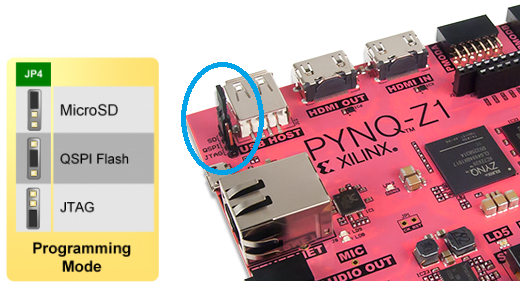
\includegraphics[width=5cm]{PIC/BootJumper}}
	\caption{Boot Jumper JP4}
	\label{Boot_Jumperr}
	\end{figure}

Die drei Startmodi werden im folgenden Text beschrieben: 

	\begin{enumerate} 
	\item   \textit{microSD Boot Mode}
	
	Der PYNQ-Z1 unterstützt \textbf{Booting} von einer microSD-Karte, die in Anschluss \textbf{J9} eingesetzt ist.
	
	\item  \textit{Quad SPI Boot Mode}
	
	Der PYNQ-Z1 verfügt über einen integrierten 16-MB-Quad-SPI-Flash, von dem der Zynq booten kann.
	
	\item  \textit{JTAG Boot Mode}
	
	Wenn der Prozessor in den JTAG-Startmodus versetzt wird, wartet er, bis die Software mithilfe der Xilinx-Tools von einem Host-Computer geladen wird.\\
Nach dem Laden der Software kann die Software entweder mit der Ausführung beginnen oder mit dem Xilinx SDK zeilenweise durchlaufen werden.
	\end{enumerate}

\subsection{microSD Slot}

Der PYNQ-Z1 bietet einen microSD-Slot\footnote{Steckplatz} (J9) für \textit{''non-volatile''} externen Speicher sowie zum Booten des Zynq.
Der Steckplatz ist mit Bank 1/501 MIO [40-47] auch einschließlich Card Detect verbunden.

	\begin{figure}[H]
	\centering
	\subfloat{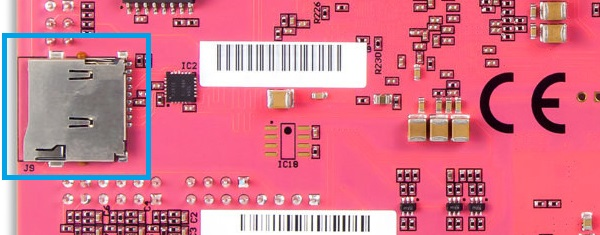
\includegraphics[width=7cm]{PIC/SDcard}}
	\caption{microSD-Slot}
	\label{microSD_Slot}
	\end{figure}
	
	
\textbf{Hinweis:} Für das Betriebssystem wird mindestens eine\textbf{ Klasse-4 Karte} mit \textbf{8 GB Speicherplatz} empfohlen.

Informationen zum Einrichten und Verwendung der Speicherkarte finden Sie im Abschnitt Software und im Bereich \textbf{\nameref{Einrichtung_der_Speicherkarte}}.



\subsection{HDMI IN/OUT}

Die PYNQ-Z1-Karte enthält einen HDMI-Eingangsanschluss und einen HDMI-Ausgangsanschluss, die mit dem FPGA-Fabric des Zynq Chips verbunden sind.
Dies bedeutet, dass zur Verwendung der HDMI-Anschlüsse die HDMI-Controller in einer Hardware-Bibliothek oder einem Overlay enthalten müssen.

	\begin{figure}[H]
	\centering
	\subfloat{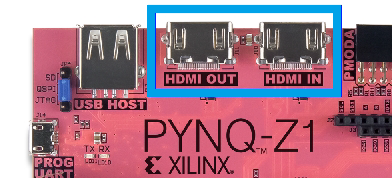
\includegraphics[width=7cm]{PIC/HDMIINOUT}}
	\caption{HDMI IN/OUT}
	\label{HDMI_IN_/_OUT}
	\end{figure}

Das Basis-Overlay enthält einen HDMI-Eingangscontroller und einen HDMI-Ausgangscontroller, die beide an die entsprechenden HDMI-Anschlüsse angeschlossen sind.\\
Am Zynq PS ist ein USB-Controller angeschlossen. Eine Webcam kann auch zum Aufnehmen von Bildern oder Videoeingaben verwendet werden, die über den HDMI-Ausgang verarbeitet und angezeigt werden können.


\subsection{USB-HOST}
Der PYNQ-Z1 implementiert eine der beiden verfügbaren PS-USB-OTG\footnote{On-The-Go}-Schnittstellen auf dem Zynq-Gerät.
Als PHY wird ein Microchip USB3320 USB 2.0 Transceiver-Chip mit einer 8-Bit-ULPI-Schnittstelle verwendet.

	\begin{figure}[H]
	\centering
	\subfloat{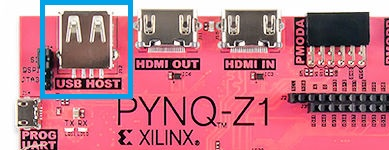
\includegraphics[width=7cm]{PIC/USBHOST}}
	\caption{USB Host}
	\label{USB_Host}
	\end{figure}

Das PHY verfügt über ein komplettes HSUSB Physical Front-End, das Geschwindigkeiten mehr als 480 MBit / s unterstützt.\\
Der PHY ist an die MIO Bank 1/501 angeschlossen, die mit 1,8 V versorgt wird. Das USB0-Peripheriegerät wird an der PS verwendet, die über MIO [28-39] angeschlossen ist.\\
\textbf{Hinweis:} USB OTG ist eine Variante des Universal Serial Bus (USB), die es einem USB-Gerät ermöglicht, eingeschränkte USB-Host-Aufgaben zu übernehmen.


\subsection{PMOD A/B}
\label{PMODE_PORTS}

Ein Pmod-Port ist eine offene 12-polige Schnittstelle, die von einer Reihe von Pmod-Peripheriegeräten unterstützt wird.\\

Typische Pmod-Peripheriegeräte sind:
	
	\begin{itemize}
		\item Sensoren (Spannung, Licht, Temperatur)
		\item Kamera
		\item Kommunikationsschnittstellen (Ethernet, seriell, WLAN, Bluetooth) 
		\item Eingangs- und Ausgangsschnittstellen (Tasten, Schalter, LEDs)
	\end{itemize}

		\begin{figure}[H]
			\centering
			\subfloat{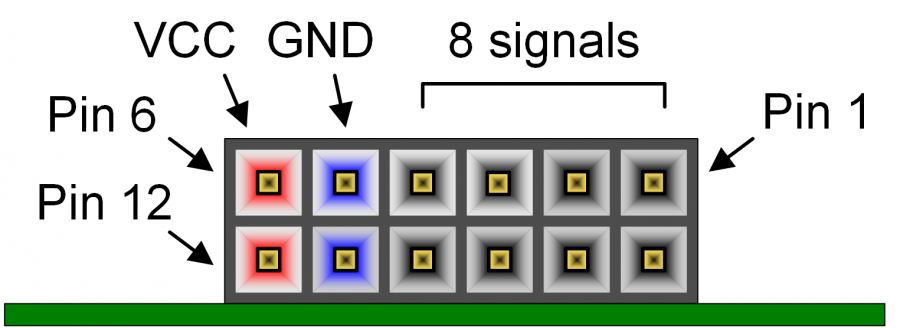
\includegraphics[width=7cm]{PIC/pynqPmod}}
			\qquad
			\subfloat{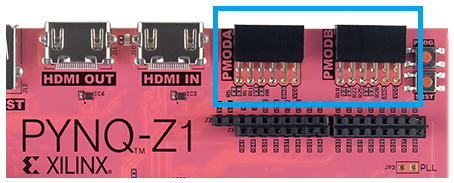
\includegraphics[width=7cm]{PIC/pmodport}}
			\caption{PYNQ PMODE Pins und PYNQ PMODE Ports }
			\label{fig:PYNQ_PMODE_PYNQ_PMODE_Ports}
		\end{figure}


	
High-Speed Pmod ports, jeder 12 Pins Pmod-Port liefert zwei 3,3 VCC Signale (Pins 6 und 12), zwei Groundssignale (Pins 5 und 11) und 8 Logiksignale.\\

\textbf{Hinweis:} Da die Pins nicht gegen Kurzschluss oder Überspannung (>3.3V) geschützt sind, muss beim Verdrahten
besonders aufgepasst werden.\\\\
Aufgrund der Verwendung dieser Komponente  im Projekt werden wird in den folgenden Kapiteln und der \textbf{\nameref{Implementierung_des_Projeks}}-Abschnitt vollständig erklärt.


\subsection{Arduino / chipKIT Shield Header}
Der PYNQ-Z1 kann an Standard-Arduino und ChipKIT Shields angeschlossen werden, um die Funktionalität zu erweitern.
Der Shield Connector verfügt über 49 Pins, die für allgemeine digitale E / A mit dem Zynq PL verbunden sind.

	\begin{figure}[H]
	\centering
	\subfloat{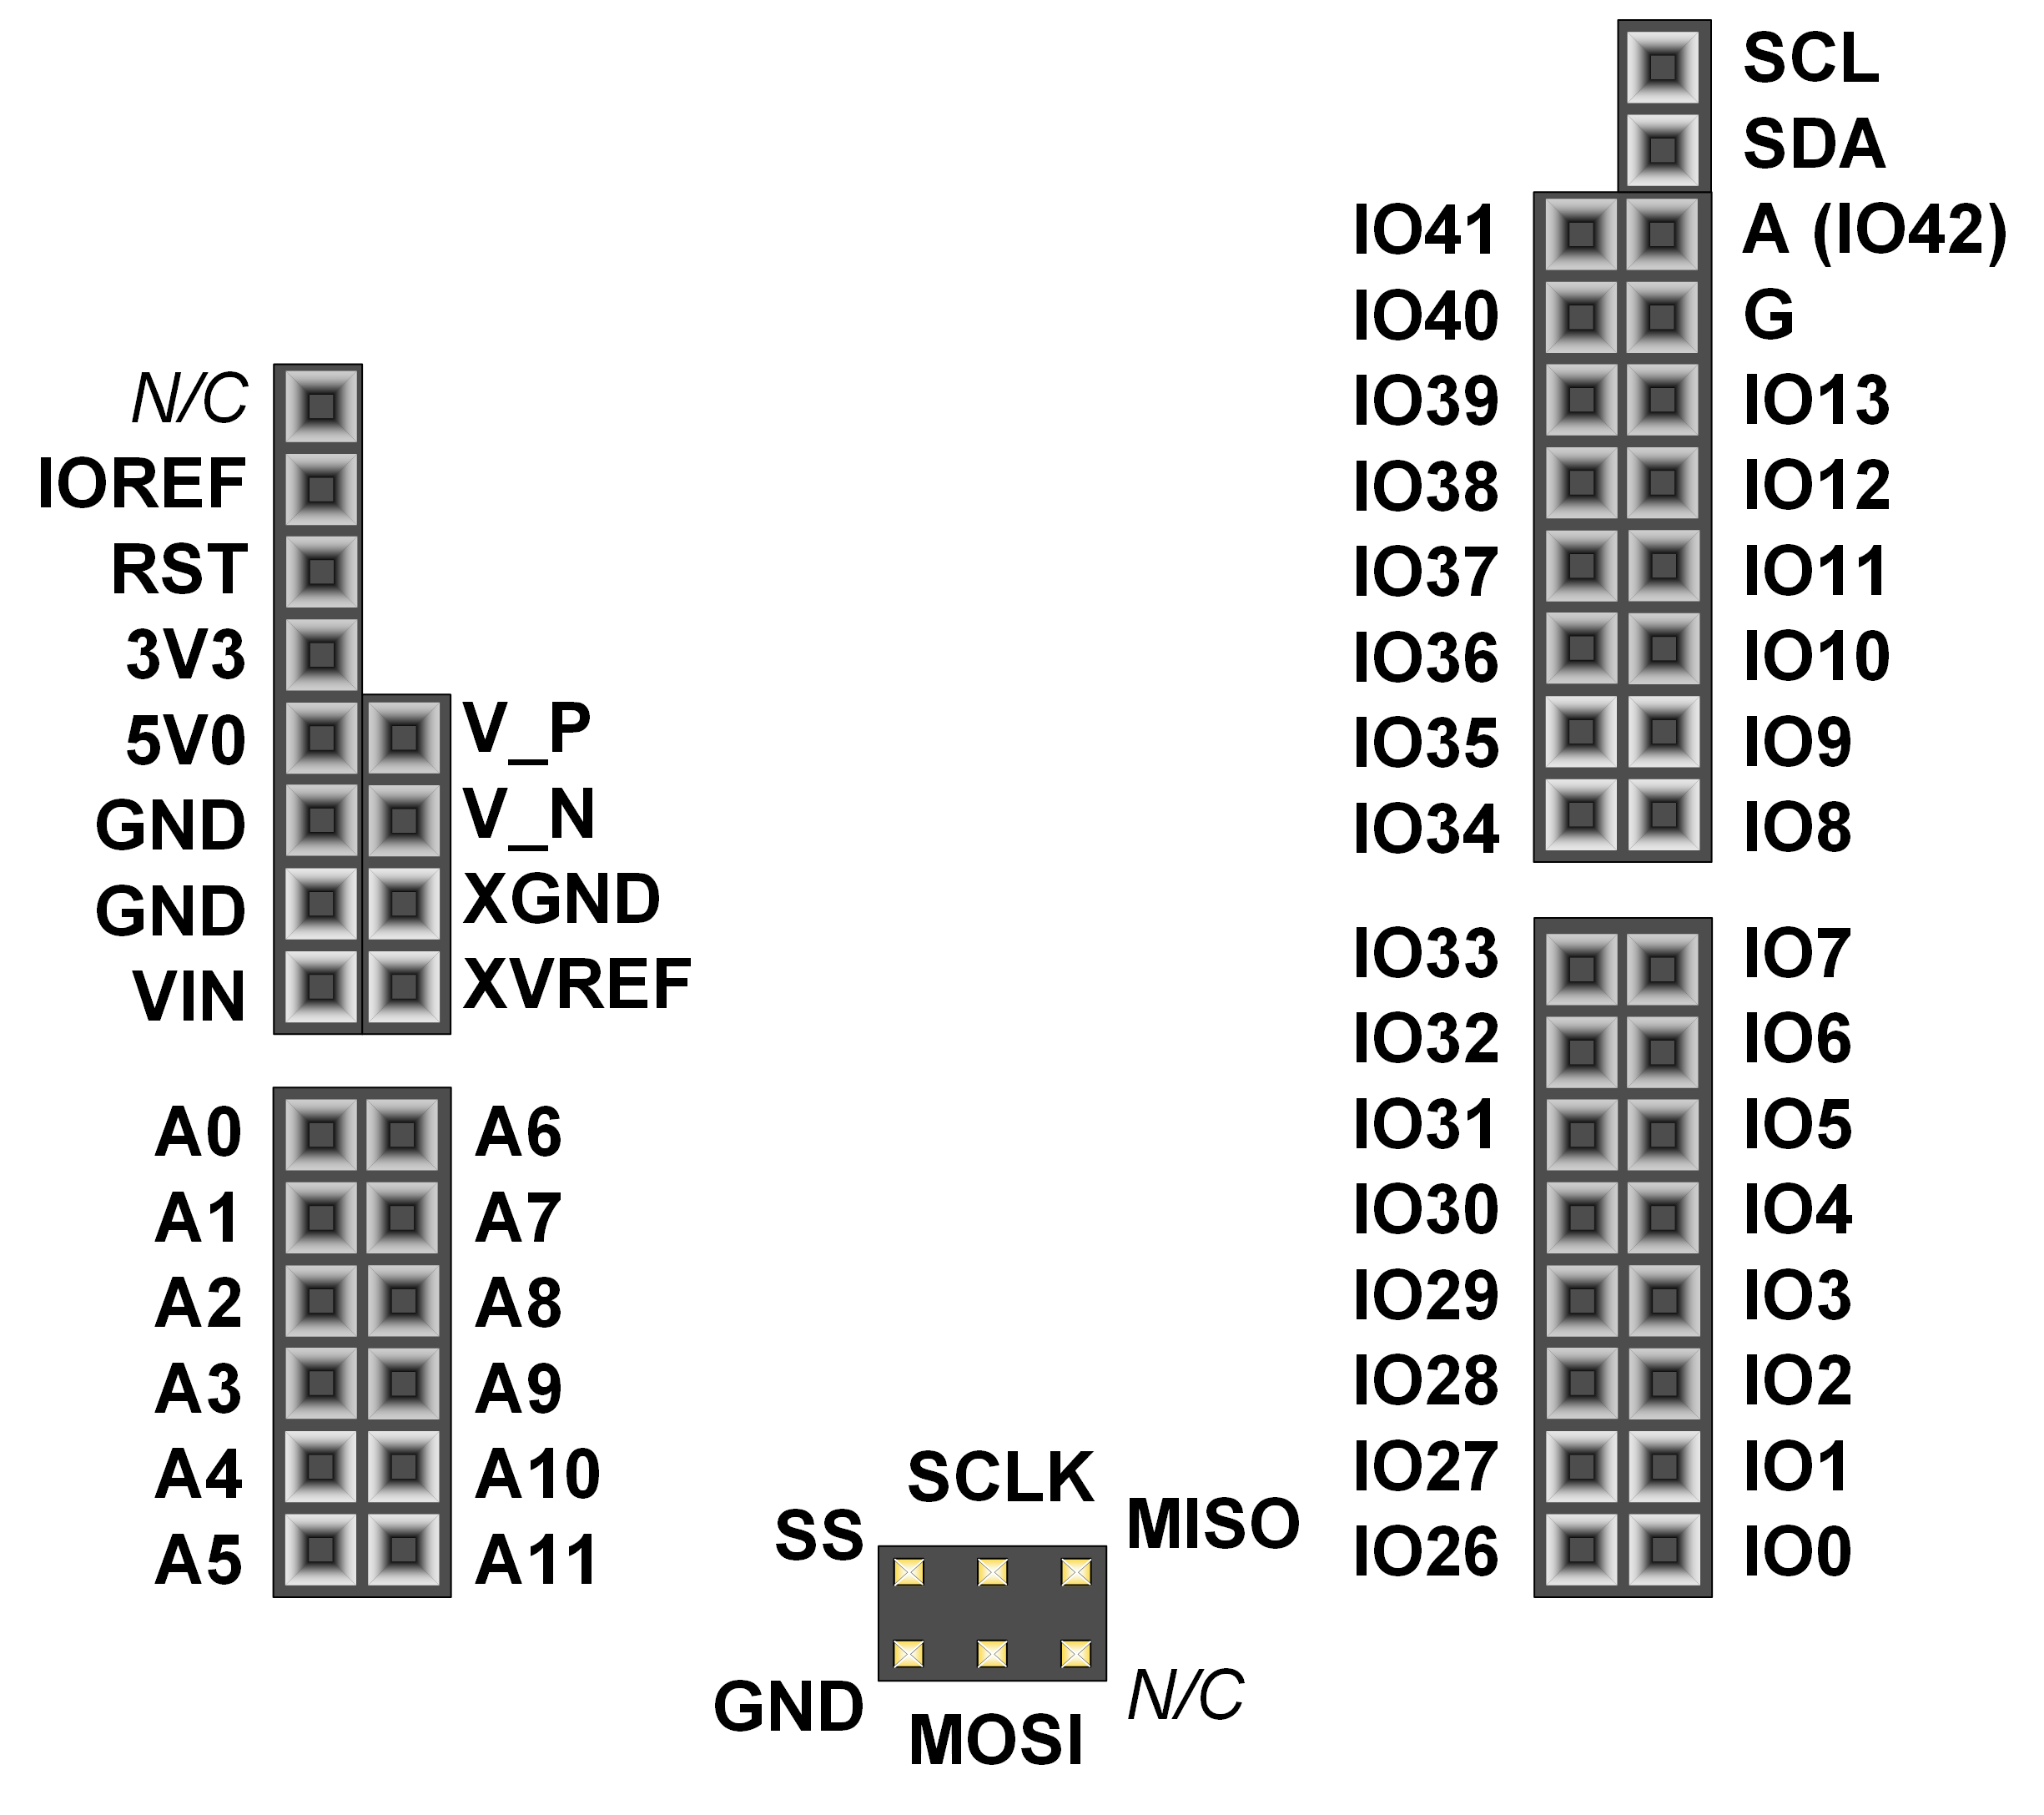
\includegraphics[width=7cm]{PIC/pynqz1shield}}
	\caption{Shield Pin Diagram}
	\label{fig:Shield_Pin_Diagram}
	\end{figure}

Aufgrund der Flexibilität von FPGAs können diese Pins für nahezu alles verwendet werden, einschließlich digitalem Lesen / Schreiben, SPI-Verbindungen, UART-Verbindungen, I2C\footnote{I-squared-C protocol}Verbindungen, VGA Controller und PWM.

6 dieser Pins (mit AN0-AN5 bezeichnet) können auch als unsymmetrische Analogeingänge mit einem Eingangsbereich von 0 V bis 3,3 V verwendet werden, und weitere 6 (mit AN6-11 bezeichnet) können als differentielle Analogeingänge verwendet werden.\\

	\textbf{Hinweis1 :} Der PYNQ-Z1 ist \textbf{nicht} mit Shield kompatibel, die 5-V-Digital- oder Analogsignale ausgeben.
	
	\textbf{Hinweis2 :}  Mehr als \textbf{5 V} kann die Driving pins am PYNQ-Z1- Shield Connector beschädigen.



\subsection{Ethernet}
Der PYNQ-Z1 verwendet einen Realtek RTL8211E-VL PHY, um einen 10/100/1000 Ethernet-Port für die Netzwerkverbindung zu implementieren.

	\begin{figure}[H]
	\centering
	\subfloat{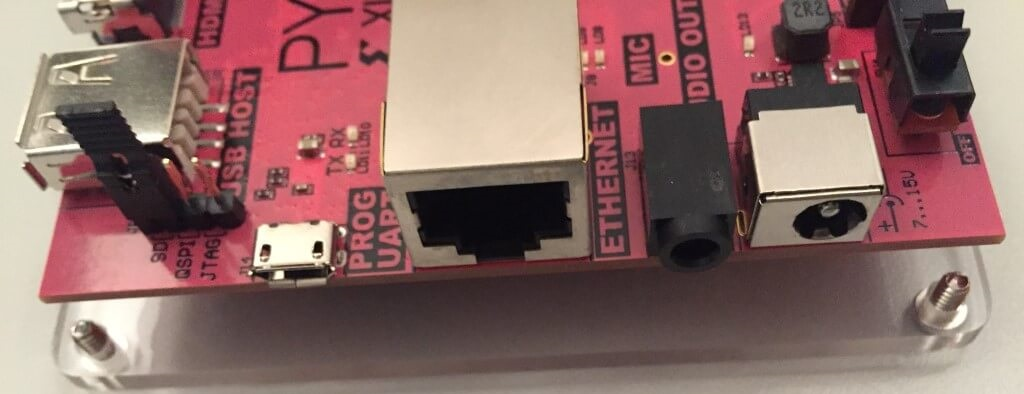
\includegraphics[width=7cm]{PIC/PYNQZ1Ethernet}}
	\caption{Ethernet}
	\label{fig:Ethernet}
	\end{figure}

Das Board versucht nach dem Anschalten über DHCP eine IP-Adresse zu erhalten und fällt auf \sout{192.168.3.99/24} 192.168.3.99:9090 zurück, falls kein DHCP Server verfügbar ist.\\

\textbf{Hinweis:} IP-Adressen Port hängt von der Version des Image Files \textbf{pynq{\_}z1{\_}v2.1.img}, z.B. bei Version 2.0 lautet 192.168.2.99:9090 und es ist möglich, dass bei einer anderen Version als 2.0 die Ip-Adresse angepasst werden muss.\\
	
Der PYNQ-Z1 enthält auch andere Komponenten wie MIC/AUDIO OUT, Schalter, Taster, RGB LEDs, u.s.w.\\\\
Weitere Informationen zu diesen Teilen finden Sie im PYNQ-Z1-Handbuch.




\section{Kamera - Ov7670}
Der OV7670 verwendet den RGB565-Modus mit 30 Bildern pro Sekunde. Die Frames können im internen BRAM\footnote{BLOCK RAM} des 7Z020 des ZYNQ7-Chips gespeichert werden. Der VGA-Controller liest die Daten aus dem Block Ram und verwendet eine 12-Bit-Farbtiefe auf dem VGA-Schnittstellenbildschirm.\\
Die VGA-Auflösung beträgt ebenfalls 640x480. Die Kamera wird mit +3,3V versorgt.

		\begin{figure}[H]
			\centering
			\subfloat{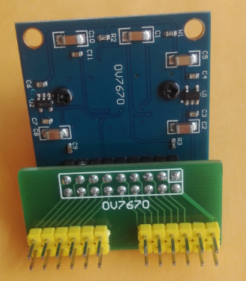
\includegraphics[width=4cm]{PIC/Ov7670camera_Back}}
			\qquad
			\subfloat{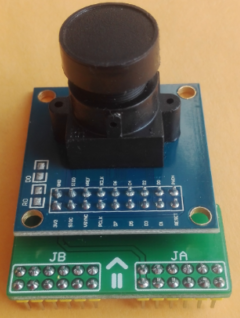
\includegraphics[width=3.45cm]{PIC/Ov7670camera_Front}}
			\caption{Kamera - Ov7670}
			\label{fig:Kamera - Ov7670}
		\end{figure}


\textbf{Hinweis: } 7Z020 verfügt über einen umfangreichen BLOCK RAM-Block, sodass Sie 640X480 = 307200 12-Bit-Nummern direkt speichern können, sodass kein externer Speicher für die Videopufferung verwendet wird.

Bemerkenswerte Eigenschaften dieser Kamera sind:
	\begin{itemize}
		\item Steuerung den SCB\footnote{Storz Communication Bus}-Busteil
		\item Broad stopband performance bis to 8 GHz
		\item Fast roll-off
		\item Connectorized package
	\end{itemize}



\section{VGA- D Adapter}
Es ist Kleine Platine mit 16 poligem Terminalblock ( Klemmleisten 3,81mm Raster) auf eine 3-reihige High Density Buchse für VGA\footnote{Video Graphics Array} Anwendungen.
VGA- D Adapter umfasst die Spezifikation einer analogen elektronischen Schnittstelle zur Übertragung von Bildern oder Videos zwischen unseren Board und Bildschirm sowie Spezifikationen für hierzu geeignete Stecker und Kabel.


		\begin{figure}[H]
			\centering
			\subfloat{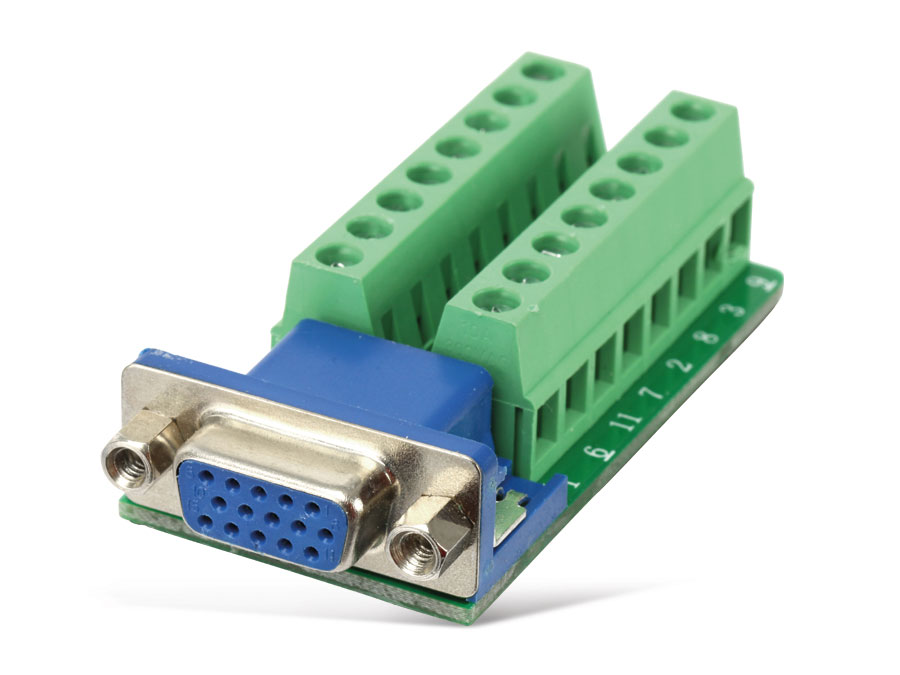
\includegraphics[width=5cm]{PIC/AdapterVGA2}}
			\qquad
			\subfloat{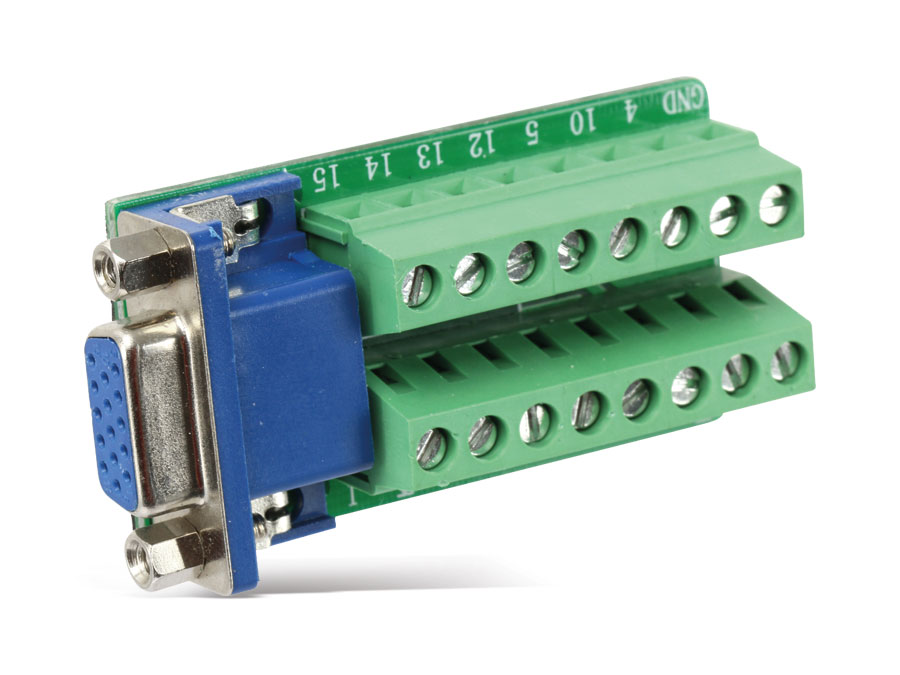
\includegraphics[width=5cm]{PIC/AdapterVGA1}}
			\caption{VGA D Adapter}
			\label{fig:VGA_Adapter}
		\end{figure}




	%------------------------------------------------
	%	3. Chapter
	%------------------------------------------------

\chapter{Softdware}

	
\section{Einrichtung der SDkarte}
\label{Einrichtung_der_SDkarte}


Mit dem folgenden Verfahren können Sie den Zynq von microSD mit einem Standard-\textbf{Zynq-Boot-Image} starten, das mit den Xilinx-Tools erstellt wurde:

	\begin{enumerate} 
	
		\item Formatieren Sie die microSD-Karte mit einem FAT32-Dateisystem.
		\item Kopieren Sie das mit Xilinx SDK erstellte \textbf{Zynq Boot Image} auf die microSD-Karte.
		\item Benennen Sie das Zynq-Boot-Image auf der microSD-Karte in\textbf{ BOOT.bin }um.
		\item Entnehmen Sie die microSD-Karte aus Ihrem Computer und stecken Sie sie in den Anschluss\textbf{ J9} des PYNQ-Z1.
		\item Schließen Sie eine\textbf{ Stromquelle} an den PYNQ-Z1 an und wählen Sie sie mit\textbf{ JP5 }aus.
		\item Stecken Sie einen einzelnen\textbf{ Jumper} auf \textbf{ JP4 } und schließen Sie die beiden oberen Stifte (mit der Bezeichnung „SD“) kurz.
		\item Schalten Sie die Karte ein. Das Board bootet nun das Image von der microSD-Karte.

	\end{enumerate}

\section{PYNQ-Z1 Installationsanleitung}
Für PYNQ-Z1-Board können Sie der Kurzanleitung folgen:


\subsection{Board Setup}

	\begin{figure}[H]
	\centering
	\subfloat{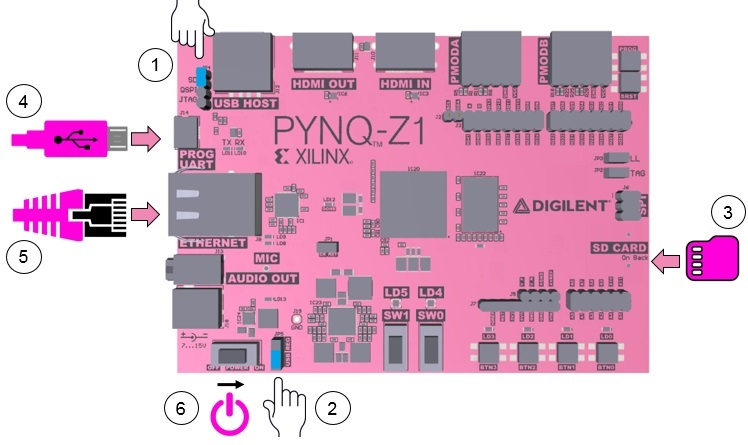
\includegraphics[width=11cm]{PIC/pynqz1setup}}
	\caption{Board Setup}
	\label{fig:Board_Setup}
	\end{figure}



	\begin{enumerate} 
		\item Setzen Sie den \textbf{JP4 / Boot-Jumper} auf die \textbf{SD-Position}, indem Sie den Jumper wie in der Abbildung gezeigt über die beiden oberen Stifte von JP4 stecken.\\
		 (Dadurch wird das Board so eingestellt, dass es von der Micro-SD-Karte bootet.)

		\item Um den PYNQ-Z1 über das Micro-USB-Kabel mit Strom zu versorgen, setzen Sie den \textbf{ JP5 / Power}-Jumper auf die USB-Position.\\
(Sie können die Karte auch über einen externen 12-V-Spannungsregler mit Strom versorgen, indem Sie den Jumper auf REG setzen.)

		\item Setzen Sie die mit dem PYNQ-Z1-Image geladene Micro-SD-Karte in den \textbf{Micro-SD}-Kartensteckplatz unter der Karte ein.

		\item Setzen Sie die mit dem PYNQ-Z1-Image geladene Micro-SD-Karte in den Micro-SD-Kartensteckplatz unter der Karte ein.

		\item Schließen Sie das USB-Kabel an Ihren PC / Laptop und an den \textbf{PROG-UART / J14} MicroUSB-Anschluss auf der Karte an.

		\item Schließen Sie die Karte an Ethernet an, indem Sie die folgenden Anweisungen befolgen.

		\item Schalten Sie den PYNQ-Z1 ein.

	\end{enumerate}



\subsection{Verbindung mit einem Rechner}
Auf Ihrem Computer muss ein Ethernet-Anschluss verfügbar sein, und Sie müssen über Berechtigungen zum Konfigurieren Ihrer Netzwerkschnittstelle verfügen. Ohne Internetzugang können Sie keine neuen Pakete aktualisieren oder laden.

	Direkt an einen Rechner anschließen (Statische IP):
		\begin{enumerate} 
		\item Geben Sie Ihren Rechner eine statische IP-Adresse
		\item Verbinden Sie die Karte mit dem Ethernet-Anschluss Ihres Computers
		\item Navigieren Sie zu \textbf{http://192.168.2.99}
		\end{enumerate}
 
\textbf{Hinweis: } Wenn obere Methode nicht klappt sein, können Sie Ihren Rechner durch '' Verbindung zu einem Netzwerk-Router'' mit dem Board verbinden. 


\subsection{Anschließen an Jupyter Notebook}

Sobald Ihr Board eingerichtet ist, öffnen Sie zum Herstellen einer Verbindung zu Jupyter Notebooks einen Webbrowser und navigieren Sie zu:\\
		
		\begin{itemize} 
		\item \textbf{http://192.168.2.99} If your board is connected to a computer via a static IP address.
		\item Wenn Ihr Board richtig konfiguriert ist, wird eine Anmeldung-Webseite angezeigt.
		Geben Sie hier den Benutzername und Passwort.
		\end{itemize}

		\begin{tcolorbox}
		Benutzername: \textbf{xilinx}\\
		Passwort: \textbf{xilinx}
		\end{tcolorbox}

Nach der Anmeldung wird der folgende Bildschirm angezeigt:

	\begin{figure}[H]
	\centering
	\subfloat{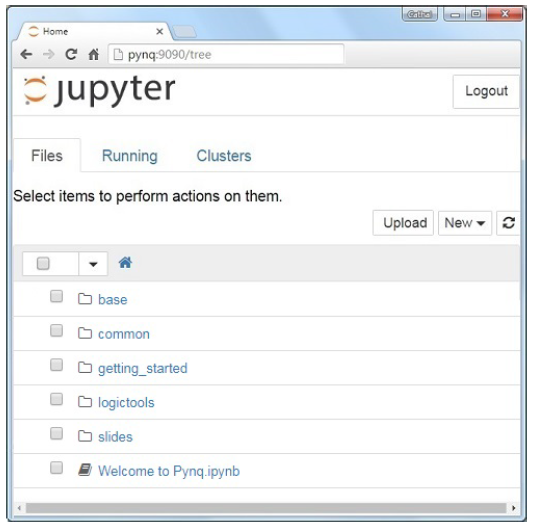
\includegraphics[width=10cm]{PIC/Jupyter}}
	\caption{Jupyter Notebook}
	\label{fig:Jupyter_Notebook}
	\end{figure}


Der Standard-Hostname lautet \textbf{pynq} und die statische Standard-IP-Adresse lautet \textbf{192.168.2.99}.

\textbf{Hinweis: } Wenn Sie die statische IP-Adresse der Karte geändert haben, müssen Sie die Adresse ändern. 



	%------------------------------------------------
	%	4. Chapter
	%------------------------------------------------

\chapter{Implementierung des Projekts}
\label{Implementierung_des_Projekts}

\section{Algorithm}
 
Zur Einschätzung des Zahlenraumes wird mit Bildgröße 640x480 gearbeitet. Bei einem Objekt von ca. 1/4 Größe des Kamerabildes muss mit ~640*480 / 4 = 76800 Pixlen im Objekt gerechnet werden. Wen das Objekt mittig liegt sind x oder y Koordinaten im Bereich $\{100,500\}$. Bei der Berechnung von $m_{02}$ wird die Spaltennummer mit sich selbst multipliziert und aufaddiert. Dies Ergibt eine Summe von $41.463.400=\{500*500+499*499+.....102*102+101*101+100*100\}$ und würde in den Wertebereich in (nicht Vorzeichen behaftete) 26Bits $2^{26}=67.108.864$. Bei  Betrachtung der gesamten Bildgröße: $87.586.240=\{640*640+639*639+.....2*2+1*1\}$ benötigt mindestens 27Bits $2^{27}=134.217.728$.
Der folgende Algorthimus zur Bestimmung der Flächenmomente bis zum Grad 2 wird vollständig in einen Int32 Datentyp passen.

 
\begin{algorithm}
\caption{Momente}
\label{Momente}
\begin{algorithmic}[1]
\Require Ein Bild $I$ mit Breite {$b$}, Höhe {$h$} und Pixelintensitäten $px\in \{I(u,v)|0,...,255\}$ $(8Bit)$. Die Laufindices $u,v,i,j,r,c \in \mathbb{N}_0$. $I$ wird als zeilenweise serialisierter Stream mit der Pixelanzahl {$L=b*h$} verarbeitet. Jedes $px$ wird als 8 separate Signalleitungen ausgelegt, die Adressierung erfolgt über $n\in \{n|0,...,7\}$ und wird als $px_n$ indiziert. Sechs Ausgabewerte {$m_{ij}\in \{m_{ij}|.0,...,2^{32}-1\}$} werden mit 0 initialisiert.

\For{$jedes$ $i$ $in$ $L$}
	\State $px = L_i$
    \If{$px_7 == 1)$}
    	\State $r=i\%b$ $(Zeile)$
    	\State $c=i/b$  $(Spalte)$
      	\State $m_{00}+=1$    
	    \State $m_{01}+= c$ 
    	\State $m_{10}+= r$
    	\State $m_{11}+= r*c$
    	\State $m_{02}+= c*c$
    	\State $m_{20}+= r*r$
    \EndIf
\EndFor
\end{algorithmic}
\end{algorithm}

\begin{algorithm}
\caption{Zentrum und Winkel der Hauptachse}
\label{Momente}
\begin{algorithmic}[1]
\Require Sechs Eingabewerte {$m_{ij}\in\{m|0,...,2^{32}-1\},ij\in\{00,01,10,11,02,20\}$} enthalten die Momente. Temporäre Variablen $\overline{x},\overline{y},\overline{x}\overline{y},\overline{x^2},\overline{y^2},\mu_{11},\mu_{02},\mu_{20}\in \{0,...,2^{32}-1\}$ und $sub,mult\in \{-2^{16},...,2^{16}-1\}$ werden mit 0 initialisiert. Ergebnisse werden als Festkommazahl $\theta \in \{+\pi, -\pi\}$ und  $\overline{x},\overline{y}$ als Zentrumkoordinaten ausgegeben.

\If{$m_{00} > 0$}
	\State $\overline{x} = \frac{m_{10}}{m_{00}}$
	\State $\overline{y} = \frac{m_{01}}{m_{00}}$
	\State $\overline{x}\overline{y} = \overline{x} * \overline{y}$
	\State $\overline{x^2} = \overline{x} * \overline{x}$
	\State $\overline{y^2} = \overline{y} * \overline{y}$
	\State $\mu_{11} = \frac{m_{11}}{m_{00}} - \overline{x}\overline{y} $
	\State $\mu_{02} = \frac{m_{02}}{m_{00}} - \overline{y}^2 $
	\State $\mu_{20} = \frac{m_{20}}{m_{00}} - \overline{x}^2 $
	\State $mult = \mu_{11}* \mu_{11}$
    \State $sub = \mu_{20}-\mu_{02}$
	\State $\theta = \frac{1}{2} atan2(mult, sub)$
\EndIf
\end{algorithmic}
\end{algorithm}

\begin{figure}[H]
\centering
\subfloat{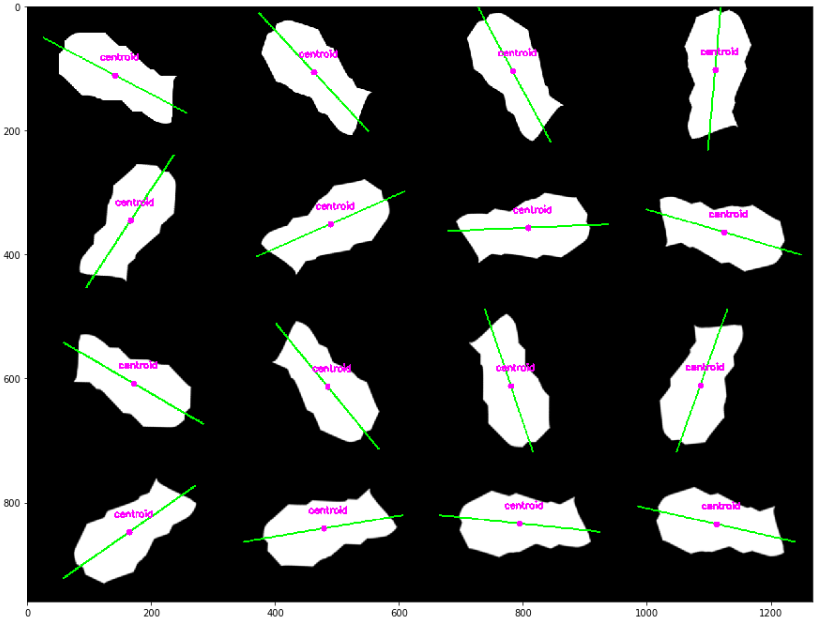
\includegraphics[width=12cm]{PIC/SimulationNumeric}}
\caption{Abbildung von Simulation-Numeric}
\label{fig:Abbildung_von_Simulation_-_Numeric}
\end{figure}

\textbf{Ergebnis von Simulation-Numeric:}
\begin{tcolorbox}
Moments: m00: 15964 m01: 1773113 m10: 2281256 m11: 269670230 m20: 365332132 m02 215154207
Center X 142.00, Center Y 111.00, Angle clockwise 27.66$^\circ$ \\

Moments: m00: 15979 m01: 1704601 m10: 2337778 m11: 268749999 m20: 369586230 m02 211883899
Center X 146.00, Center Y 106.00, Angle clockwise 47.24 $^\circ$ \\	

Moments: m00: 15975 m01: 1662657 m10: 2398584 m11: 265651241 m20: 377952942 m02 212836887
Center X 150.00, Center Y 104.00, Angle clockwise 61.61 $^\circ$ \\
\end{tcolorbox}

\textbf{Anpassung des Winkelergebnisses, atan2 mit positiven Argumenten:}
Es erfolgt eine Gegenüberstellung von dem Ergebnis der atan2 Funktion mit Argumenten, die einmal mit korrektem Vorzeichen verwendet werden und einmal mit ihrem Absolutwert. Bei Verwendung des Absolutwertes muss das Ergebnis nochmal korrigiert werden.
\begin{tcolorbox}
$mult = \mu_{11}* \mu_{11}$ versus $mult = abs(\mu_{11}* \mu_{11})$ Ergebnis mit $abs$ gekennzeichnet\\
$sub = \mu_{20}-\mu_{02}$ versus $sub = abs(\mu_{20}-\mu_{02})$ Ergebnis mit $abs$ gekennzeichnet\\
$\theta = \frac{1}{2} atan2(mult, sub)$\\
sub: -1348.09 mul: 2058.37 Center X 150.00, Center Y 104.00, Angle atan2 61.61$^\circ$  \\
korrekt: -s+m=61.61$^\circ$, abs: +s+m: 28.39$^\circ$, Anpassung: (90$^\circ$-x)\\

sub: -887.58 mul: -2094.80 Center X 167.00, Center Y 105.00, Angle atan2 -56.48$^\circ$ \\
korrekt: -s-m=-56.48$^\circ$, abs: +s+m: 33.52$^\circ$, Anpassung: (x+90$^\circ$ )\\

sub: 1435.64 mul: -1549.62 Center X 173.00, Center Y 111.00, Angle atan2 -23.59$^\circ$ \\
korrekt: +s-m=-23.59$^\circ$, abs: +s+m: 23.59$^\circ$, Anpassung: (x*(-1$^\circ$))\\
\end{tcolorbox}

\begin{algorithm}
\caption{Zentrum und Winkel der Hauptachse mit abs(mult) und abs(sub)}
\label{Momente}
\begin{algorithmic}[1]
\Require Sechs Eingabewerte {$m_{ij}\in\{m|0,...,2^{32}-1\},ij\in\{00,01,10,11,02,20\}$} enthalten die Momente. Temporäre Variablen $\overline{x},\overline{y},\overline{x}\overline{y},\overline{x^2},\overline{y^2},\mu_{11},\mu_{02},\mu_{20},sub,mult\in \{0,...,2^{32}-1\}$ werden mit 0 initialisiert. Ergebnisse werden als Festkommazahl $\theta \in \{+\pi, -\pi\}$ und  $\overline{x},\overline{y}$ als Zentrumkoordinaten. Flags $s,m$ für Korrektur des Ergebnisses $\theta$. {$s,m\in\{0,1\}$} ausgegeben.
\State $m = 0$, $s = 0$
\If{$m_{00} > 0$}
	\State $\overline{x} = \frac{m_{10}}{m_{00}}$
	\State $\overline{y} = \frac{m_{01}}{m_{00}}$
	\State $\overline{x}\overline{y} = \overline{x} * \overline{y}$
	\State $\overline{x^2} = \overline{x} * \overline{x}$
	\State $\overline{y^2} = \overline{y} * \overline{y}$
	\State $\mu_{11} = \frac{m_{11}}{m_{00}} - \overline{x}\overline{y} $
	\State $\mu_{02} = \frac{m_{02}}{m_{00}} - \overline{y}^2 $
	\State $\mu_{20} = \frac{m_{20}}{m_{00}} - \overline{x}^2 $	
	\If{$\mu_{11} < 0$}
		\State $m = 1$
		\State $\mu_{11} = -\mu_{11}$
	\EndIf
	\State $mult = \mu_{11}* \mu_{11}$
	\If{$\mu_{02} < \mu_{20}$}
		\State $sub = \mu_{20}-\mu_{02}$
		\State $s = 1$
	\Else
		\State $sub = \mu_{02}-\mu_{20}$
    \EndIf  
	\State $\theta = \frac{1}{2} atan2(mult, sub)$
\EndIf
\If{$m = 1$ \&\& $s = 1$}
	\State $\theta = \theta + \frac{\pi}{2}$
\ElsIf {$m = 0$ \&\& $s = 1$}
	\State $\theta = \frac{\pi}{2} - \theta$
\ElsIf {$m = 1$ \&\& $s = 0$}
	\State $\theta= \theta*(-1)$
\EndIf  


\end{algorithmic}
\end{algorithm}

\newpage
\section{Hardware Implementierung}

\subsection{Einstellung von Pmod port}
Wie im Abschnitt \textbf{\nameref{PMODE_PORTS}} schon erwähnt wurde, 


\section{HLS Software Implementierung}
In dieser Sektion wird eine grundlegende Einführung in die High Level Synthesis erläutet. (HLS)\\
 \textbf{Was bedeutet HLS?}\\
 High Level Synthesis wurde eingeführt, um die Elektronikkenntnisse zu reduzieren, die zum Entwerfen von Hardware erforderlich sind. Dies erleichtert auch den Ablauf des Hardware-Designs, wenn es darum geht, ein bestimmtes Verhaltensmodell zu erreichen.\\
 Unter Verwendung einer Programmiersprache wie C / C ++ implementieren wir das Verhaltensmodell in Hardware. \\
 Das HLS-Tool bildet unser Verhaltensmodell in Hardware ab und generiert den HDL-Code dafür und dann wird synthetisiert und danach im letzten Schritt wird  auf einem FPGA implementiert.


Wenn Wir mit HLS vertraut sind, fahren wir mit dem Beginn der Schritte fort und erzeugen unseren eigenen  \textbf{IP Core}.
\subsection{Mein eigener IP Core}
Im ersten Schritt werden wir dies Thema nachvollziehen, dass wie ich meinen eigenen IP Core in HLS  erstellen kann!\\


\textbf{Schritt 1:} \textit{Erstellung eines neuen Projekts}\\

- Öffnen wir Vivado HLS und legen wir ein neues Projekt mit dem eigenen Funktionsnamen z.B. \textbf{„XXXX“} an.\\

- Wählen wir ein Bauteil oder eine Entwicklungsplatine aus (wir verwenden PYNQ-Z1) und beenden wir die Erstellung des neuen Projekts.\\

- Behalten wir vorerst den Standardzeitraum (10ns) bei. (Wir können ihn später ändern, wenn wir wollen.)\\

- Auf der rechten Seite des Fensters sehen wir den ''Explorer'', wie in der folgenden Abbildung.\\

\begin{figure}[H]
\centering
\subfloat{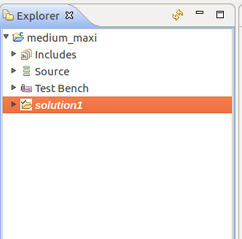
\includegraphics[width=6cm]{PIC/Explorer}}
\caption{Explorer}
\label{fig:Explorer}
\end{figure}

- Klicken wir mit der rechten Maustaste auf die Quelle, erstellen eine neue Datei, nennen wir sie mit dem eigenen Name z.B. \textbf{''core.cpp''} und speichern wir sie im Projektordner.\\
 
- Nach dem Speichern öffnet Vivado HLS automatisch die leere neue Datei. \\

 \textbf{Beginnen wir mit dem Entwerfen des IP-Cores}\\

\textbf{Schritt 2:} \textit{Entwurf des IP-Cores}\\

In diesem Schritt wird der IP-Core nur für Funktionstests entworfen. Diese Funktion muss mit Ihrem Top-Funktionsnamen benannt werden. Damit der Entwurf des IP-Kerns abgeschlossen wird, benötigen wir jedoch zum Test einen Test Bench, ob die Funktionalität des IP-Cores unseren Erwartungen entspricht.\\

\textbf{Schritt 3:} \textit{Entwurf des Test-Benchs}\\

- Erstellen wir eine neue Datei unter Test bench. Wir können die Top-Funktion (bei uns z.B. „XXXX“) in der Hauptfunktion des Test Benchs aufrufen und Ein- und Ausgänge weitergeben und prüfen.\\

- In der Hauptfunktion "test bench" ist die Rückgabe von \textbf{0} sehr wichtig, weil Vivado HLS damit prüft, ob die Funktionssimulation erfolgreich war.\\

\textbf{Schritt 4:} \textit{Ausführung des Test Benchs für Verhaltenssimulation}\\

- Führen wir unseren Test Bench aus. Klicken wir in der oberen \textit{Toolbar} auf \textbf{''Run C Simulation''}.

- Dann wird ''Popup-Window'' wie in der folgenden Abbildung angezeigt:\\

\begin{figure}[H]
\centering
\subfloat{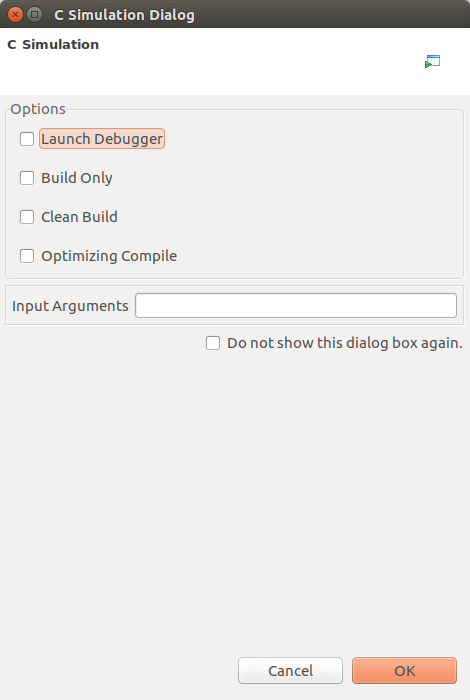
\includegraphics[width=6cm]{PIC/popupwindow}}
\caption{C-Simulation pop-up Fenster}
\label{fig:C_Simulation_pop_-_up_Fenster}
\end{figure}

- Wählen wir hier einfach ''OK'' und die \textit{C-Simulation} wird gestartet. Dies wird einige Zeit (abhängig von Ihren Ressourcen) nehmen.\\

\textbf{Schritt 5:} \textit{Vorbereitung des IP-Cores für die Synthese}\\

Wir können \textit{Compiler-Directives} verwenden, um den Compiler dazu zu bringen, den IP-Core so zu synthetisieren.\\

Wenn wir keine Compiler-Directives verwenden, analysiert \textit{Vivado HLS} den Code und verwendet Standard-Directives an den entsprechenden Positionen des Codes. Wir können diese Standardanweisungen im rechten Fenster unter der Registerkarte  \textbf{''Directive''} sehen.\\

Mit Doppelklick auf ''Ein- oder Ausgänge'' wird Ein Fenster angezeigt, dass wir die Optionen wie in der folgenden Abbildung ausfüllen können und dass klicken wir auf ''OK''.\\


\begin{figure}[H]
\centering
\subfloat{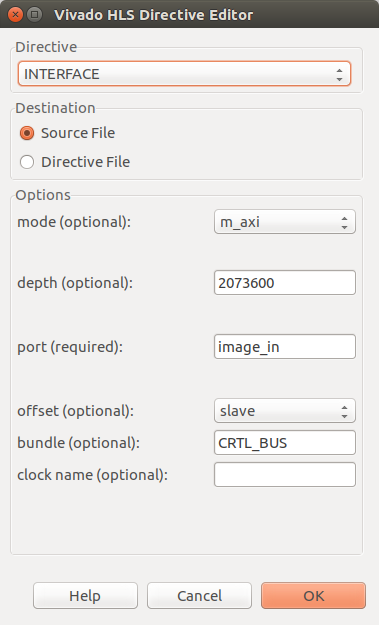
\includegraphics[width=6cm]{PIC/VivadoHLSDirectiveEditor}}
\caption{Vivado HLS Directive Editor}
\label{fig:Vivado_HLS_Directive_Editor}
\end{figure}



	\begin{itemize}
		\item  \textbf{directive}
		
		Interface, da wir Eingabe-Ausgabeschnittstelle für den IP-Core verwenden wollen.
		
		\item  \textbf{mode}
		
		Es steht für einen AXI oder AXI Master Full-Port.

		\item  \textbf{depth}

		Größe des Arrays. Dies ist optional. Wenn wir dieses Feld leer lassen, verwendet Vivado HLS die Standardtiefe. Es ist besser, wenn wir hier die Tiefe angeben können. Durch Auswahl von ''Slave'' können wir die Speicheradresse des Ports zum \textit{Run-time} über einen AXI Lite-Port festlegen.
		
		\item  \textbf{offset}
		
		Hier wird \textit{''mapped memory location''} des angeschlossenen Eingangs oder Ausgangs gesteuert.
				
		\item  \textbf{bundle}
		
		Über AXI Lite wird der Port mit dem Namen \textit{''CRTL\_BUS''} gebündelt.
		
	\end{itemize}


Wählen wir dann \textbf{OK}.\\

Zum Synthetisieren des unseren IP-Cores klicken wir auf \textit{''Run C Synthesis''}.\\

Wenn das Design ordnungsgemäß synthetisiert wurde, wird ein ähnlicher Synthesebericht angezeigt.\\

\begin{figure}[H]
\centering
\subfloat{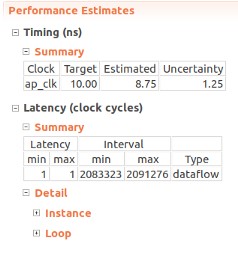
\includegraphics[width=6cm]{PIC/TimingDetails}}
\caption{Beispiel von Timing Details}
\label{fig:Beispiel_von_Timing_Details}
\end{figure}

\begin{figure}[H]
\centering
\subfloat{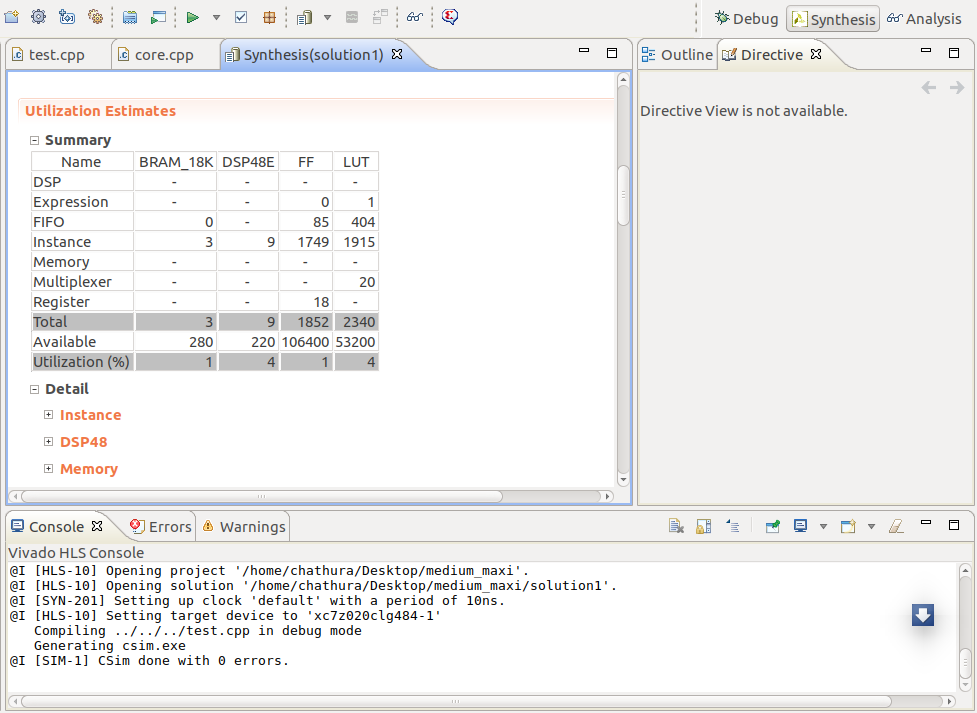
\includegraphics[width=10cm]{PIC/RessourcennutzungdesDesigns}}
\caption{Beispiel von Ressourcennutzung des Designs}
\label{fig:Ressourcennutzung_des_Designs}
\end{figure}


Bevor wir unseren IP-Core exportieren, müssen wir eine \textbf{RTL-Co-Simulation} durchführen, um die Funktionsunterschiede zwischen der \textbf{C-Simulation} und der \textbf{RTL-Simulation} zu überprüfen.

Klicken wir auf \textbf{''Run C/RTL co-simulation''} und dann klicken im Popup-Fenster auf \textbf{''OK''}, wenn \textbf{''setup only''} aktiviert ist.\\

\begin{figure}[H]
\centering
\subfloat{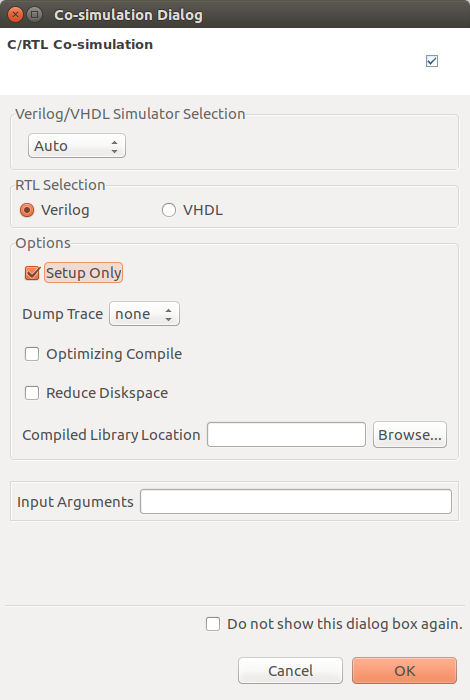
\includegraphics[width=7cm]{PIC/co-simulation}}
\caption{Beispiel von Co-Simulation}
\label{fig:Co_-_Simulation}
\end{figure}


Nachdem wir diese Simulation erfolgreich geschafft haben, können wir mit dem Export des IP-Cores vorgehen.
Klicken wir auf \textbf{''Export RTL''} und dann auf \textbf{''OK''}.\\

\begin{figure}[H]
\centering
\subfloat{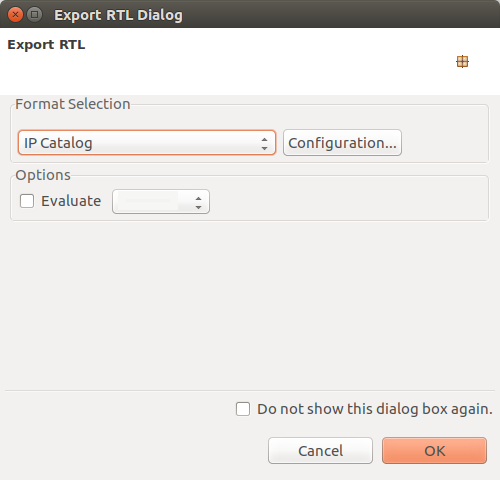
\includegraphics[width=8cm]{PIC/ExportRTL}}
\caption{Beispiel von Export RTL}
\label{fig:Export_RTL}
\end{figure}


Im obigen Fenster können wir auswählen, ob wir unser Design mithilfe einer HDL oder Verilog bewerten möchten.
Nach dem Export unseres IP-Cores sind wir mit dem IP-Core-Design mit Vivado HLS fertig.\\

Der nächste Schritt besteht darin, die gesamte Hardware-Architektur einschließlich unseres IP-Cores mit Vivado zu entwerfen.



\section{Code, Listings}

\subsection{Simulation in OpenCV}

\begin{lstlisting}[language=Python, caption=Simulation in OpenCV]      
import cv2
import numpy as np 
import sys
import math

img = cv2.imread("img.png",0)
# convert the grayscale image to binary image
ret,thresh = cv2.threshold(img,127,255,0)
# find contours in the binary image
im2, contours, hierarchy = cv2.findContours(\
	thresh,cv2.RETR_TREE,cv2.CHAIN_APPROX_SIMPLE)

print('Number contours:',len(contours))
for c in contours:
    area = cv2.contourArea(c)
    print(area)
	if (area < 100.0):
		contours.remove(c)
	print('Number contours>100:',len(contours))

cv2.namedWindow("main", cv2.WINDOW_NORMAL)
color_image = cv2.cvtColor(img, cv2.COLOR_GRAY2RGB)
cv2.drawContours(color_image, contours, -1, (0, 0, 255), 1) 

for c in contours:
    # calculate moments for each contour
    M = cv2.moments(c)

    # calculate x,y coordinate of center
    cX = int(M["m10"] / M["m00"])
    cY = int(M["m01"] / M["m00"])
   
    # cv2.circle(img, (cX, cY), 5, (255, 0, 255), -1)
    cv2.circle(color_image, (cX, cY), 5, (255, 0, 255), -1)
    cv2.putText(color_image, "centroid", (cX - 25, cY - 25),\
    	cv2.FONT_HERSHEY_SIMPLEX, 0.5, (255, 0, 255), 2)

    # display the image
    cv2.imshow("main", color_image)
    cv2.waitKey(0)
    
for c in contours:
    M = cv2.moments(c)
    cX = int(M["m10"] / M["m00"])
    cY = int(M["m01"] / M["m00"])
    mu11 = (M["m11"]/M["m00"])-(cX*cY)
    mu02 = (M["m02"]/M["m00"])-(cY**2)
    mu20 = (M["m20"]/M["m00"])-(cX**2)
    theta = 0.5 *  math.atan2( (2*mu11) , (mu20-mu02) )
      
    length = 50
    x2 = cX + length * math.cos(theta)
    y2 = cY + length * math.sin(theta) 
    lineThickness = 2
    cv2.line(color_image, (int(cX), int(cY)), (int(x2), \
    	int(y2)), (0,255,0), lineThickness)
    
# display the image
cv2.imshow("main", color_image)
cv2.waitKey(0)    
cv2.destroyAllWindows()
\end{lstlisting}

Die Abbildung vom Beispiel ''Blobs mit Schwerpunkt und Richtung'' wurde im  Abschnitt \textbf{ \nameref{Projektbeschreibung}} gezeigt.\\

\subsection{Simulation Numeric}

\begin{lstlisting}[language=Python, caption=Simulation Numeric]
import cv2
import numpy as np 
import math # for tan
import matplotlib.pyplot as plt

def calcmoments(img):
    # function to calculate moments
    moments = np.zeros(6, dtype=int) # Moments :[m00,m01,m10,m11,m20,m02]
    for y in range(img.shape[0]):
        for x in range(img.shape[1]):
            if (img[y,x] & 128): \
            	# check if 7th bit is '1', it is set for gray values >=128
                moments[0] += 1
                moments[1] += y
                moments[2] += x
                moments[3] += x*y
                moments[4] += y*y
                moments[5] += x*x
    return moments
    
def calcthetacXcY(m):
    # calculate cX,cY,theta of blob
    cxytheta = np.zeros(3, dtype=float) # cxytheta : [ cX, cY, theta ]
    cxytheta[0] = int(m[2]/m[0])
    cxytheta[1] = int(m[1]/m[0])
    mu20 = (m[4]/m[0])-cxytheta[0]**2
    mu11 = (m[3]/m[0])-cxytheta[0]*cxytheta[1]
    mu02 = (m[5]/m[0])-cxytheta[1]**2
    cxytheta[2] = 0.5 *  math.atan2((2*mu11),(mu20-mu02))
    return cxytheta
    
test = cv2.imread('pics/Block0.png',0)
tiles = 4
rows = test.shape[0]
cols = test.shape[1]
hugeImg = np.zeros( (4*rows, 4*cols, 3), np.uint8)

for i in np.arange(16):
    img = cv2.imread('pics/Block'+str(i)+'.png',0)
    m = calcmoments(img) # Moments : [ m00, m01, m10, m11, m02, m20 ]
    cxytheta = calcthetacXcY(m) # cxytheta : [ cX, cY, theta ]

    # visu, create line through center point
    length = 130
    x1 = cxytheta[0] + length * math.cos(cxytheta[2])
    y1 = cxytheta[1] + length * math.sin(cxytheta[2]) 
    x2 = cxytheta[0] - length * math.cos(cxytheta[2])
    y2 = cxytheta[1] - length * math.sin(cxytheta[2]) 
 
    color_image = cv2.cvtColor(img, cv2.COLOR_GRAY2RGB)
    lineThickness = 2
    cv2.line(color_image, (int(x1), int(y1)), (int(x2), int(y2)),\
    	(0,255,0), lineThickness)
    cv2.circle(color_image, (int(cxytheta[0]), int(cxytheta[1])), \
    	5, (255, 0, 255), -1)
    cv2.putText(color_image, "centroid", (int(cxytheta[0])-25, \
    	int(cxytheta[1])-25),cv2.FONT_HERSHEY_SIMPLEX,0.5,(255,0,255),2)
    
    # copy images into large result image
    rpos = int(i/4)*rows
    cpos = i%4*cols
    hugeImg[rpos:rpos+rows, cpos:cpos+cols] = color_image

# display plot in notebook
%matplotlib inline
plt.axis("off")
plt.figure(figsize=(15,15))
plt.imshow(hugeImg)
plt.show()

\end{lstlisting}

%------------------------------------------------
%	Literaturverzeichnis
%------------------------------------------------
\begin{thebibliography}{9}

\bibitem{PYNQ-Z1 Board} 
Xilinx PYNQ Z1 Board,
\\\texttt{https://blog.digilentinc.com/python-zynq-pynq-introducing-our-latest-collaborationl}

\bibitem{PYNQ-Z1} 
PYNQ Z1-Komponenten,
\\\texttt{https://buildmedia.readthedocs.org/media/pdf/pynq/v1.4/pynq.pdf}

\bibitem{PYNQ-Z1}
PYNQ Z1-Einrichtung,
\\\texttt{Pynq{\_}Labor{\_}Doku{\_}Jaschko{\_}Stolle.pdf}

\bibitem{Ov7670camera} 
Ov7670camera,
\\\texttt{http://www.alselectro.com/arduino-camera-ov7670.html}

\bibitem{PYNQ-Z1} 
Board Setup,
\\\texttt{pynqZ1{\_}v205.pdf}


\end{thebibliography}




\end{document}